\begin{frame}
  \frametitle{Visualisierung}
  \Wider{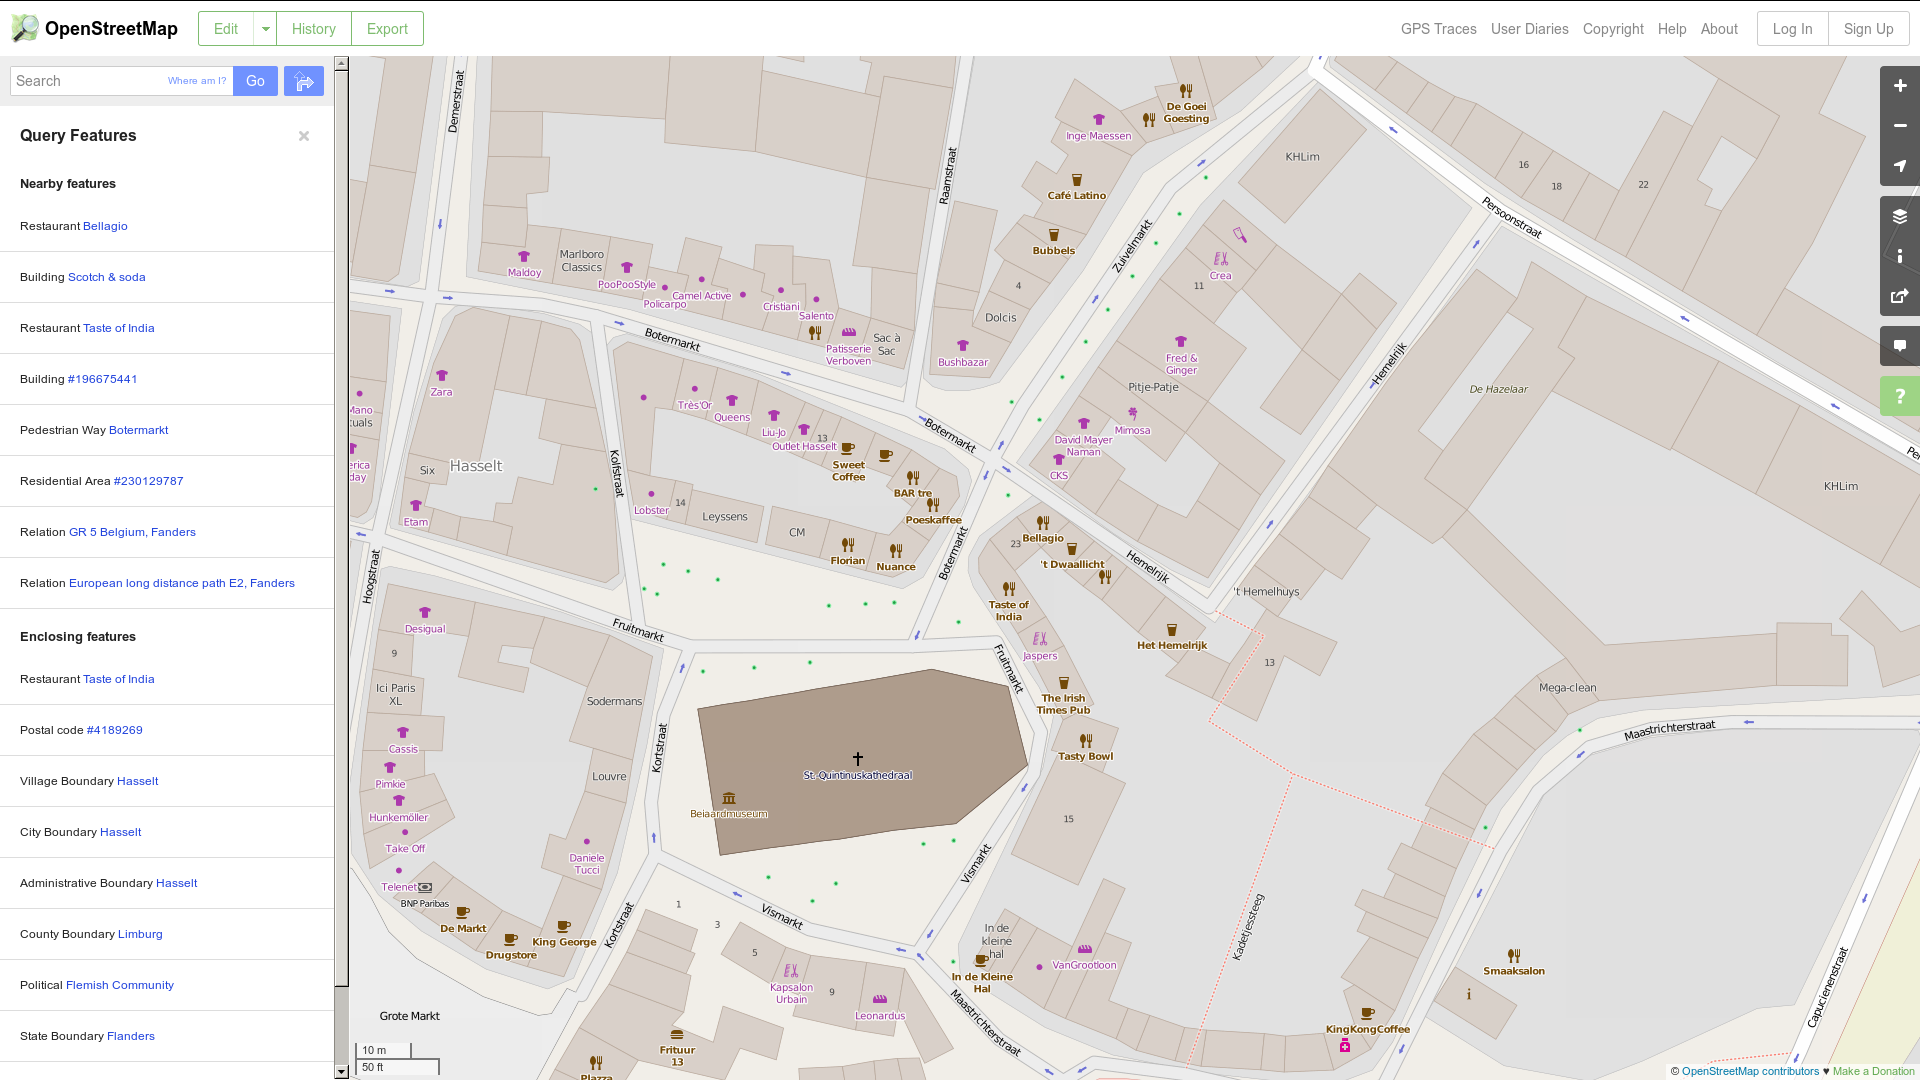
\includegraphics[width=\textwidth]{OSM_feature}}
\end{frame}

\begin{frame}[fragile]
  \frametitle{Visualisierung}
  \lstset{language=XML,basicstyle=\tiny}
  \lstinputlisting{OSM.xml}
\end{frame}

\begin{frame}
  \frametitle{Visualisierung}
  \Wider{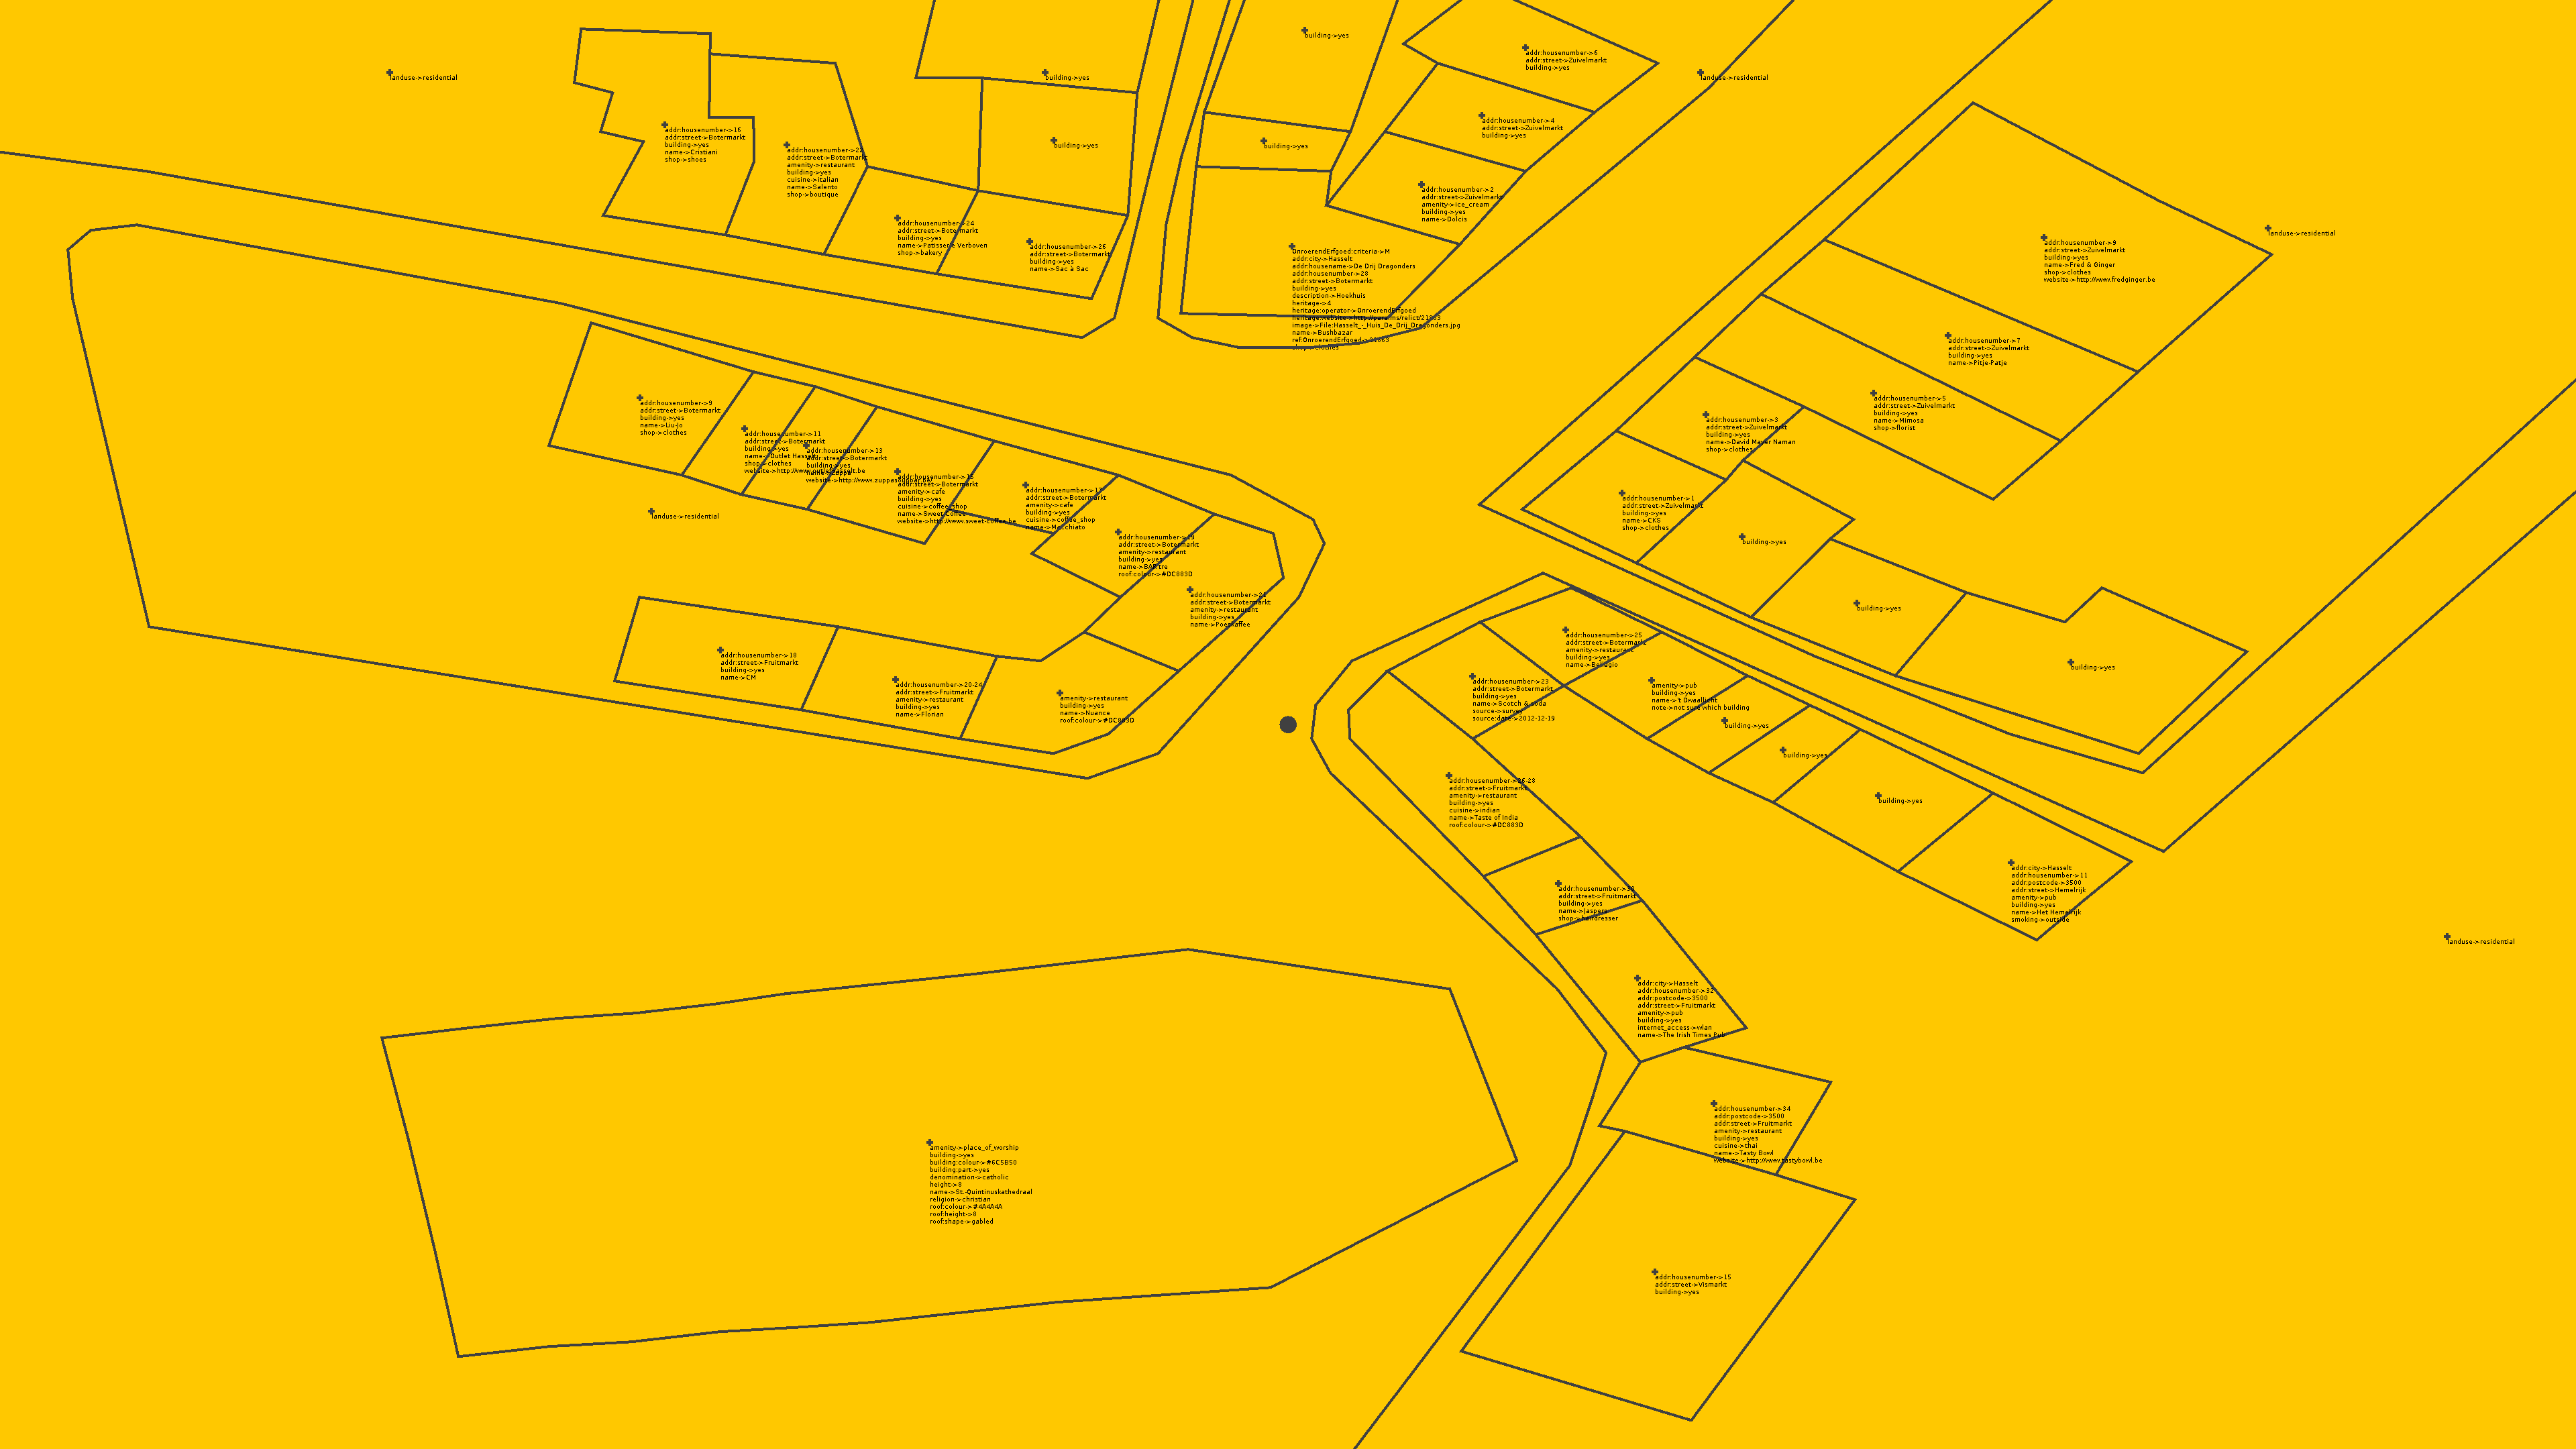
\includegraphics[width=\textwidth]{DataDrawer_raw}}
\end{frame}

\begin{frame}
  \frametitle{Visualisierung}
  \Wider{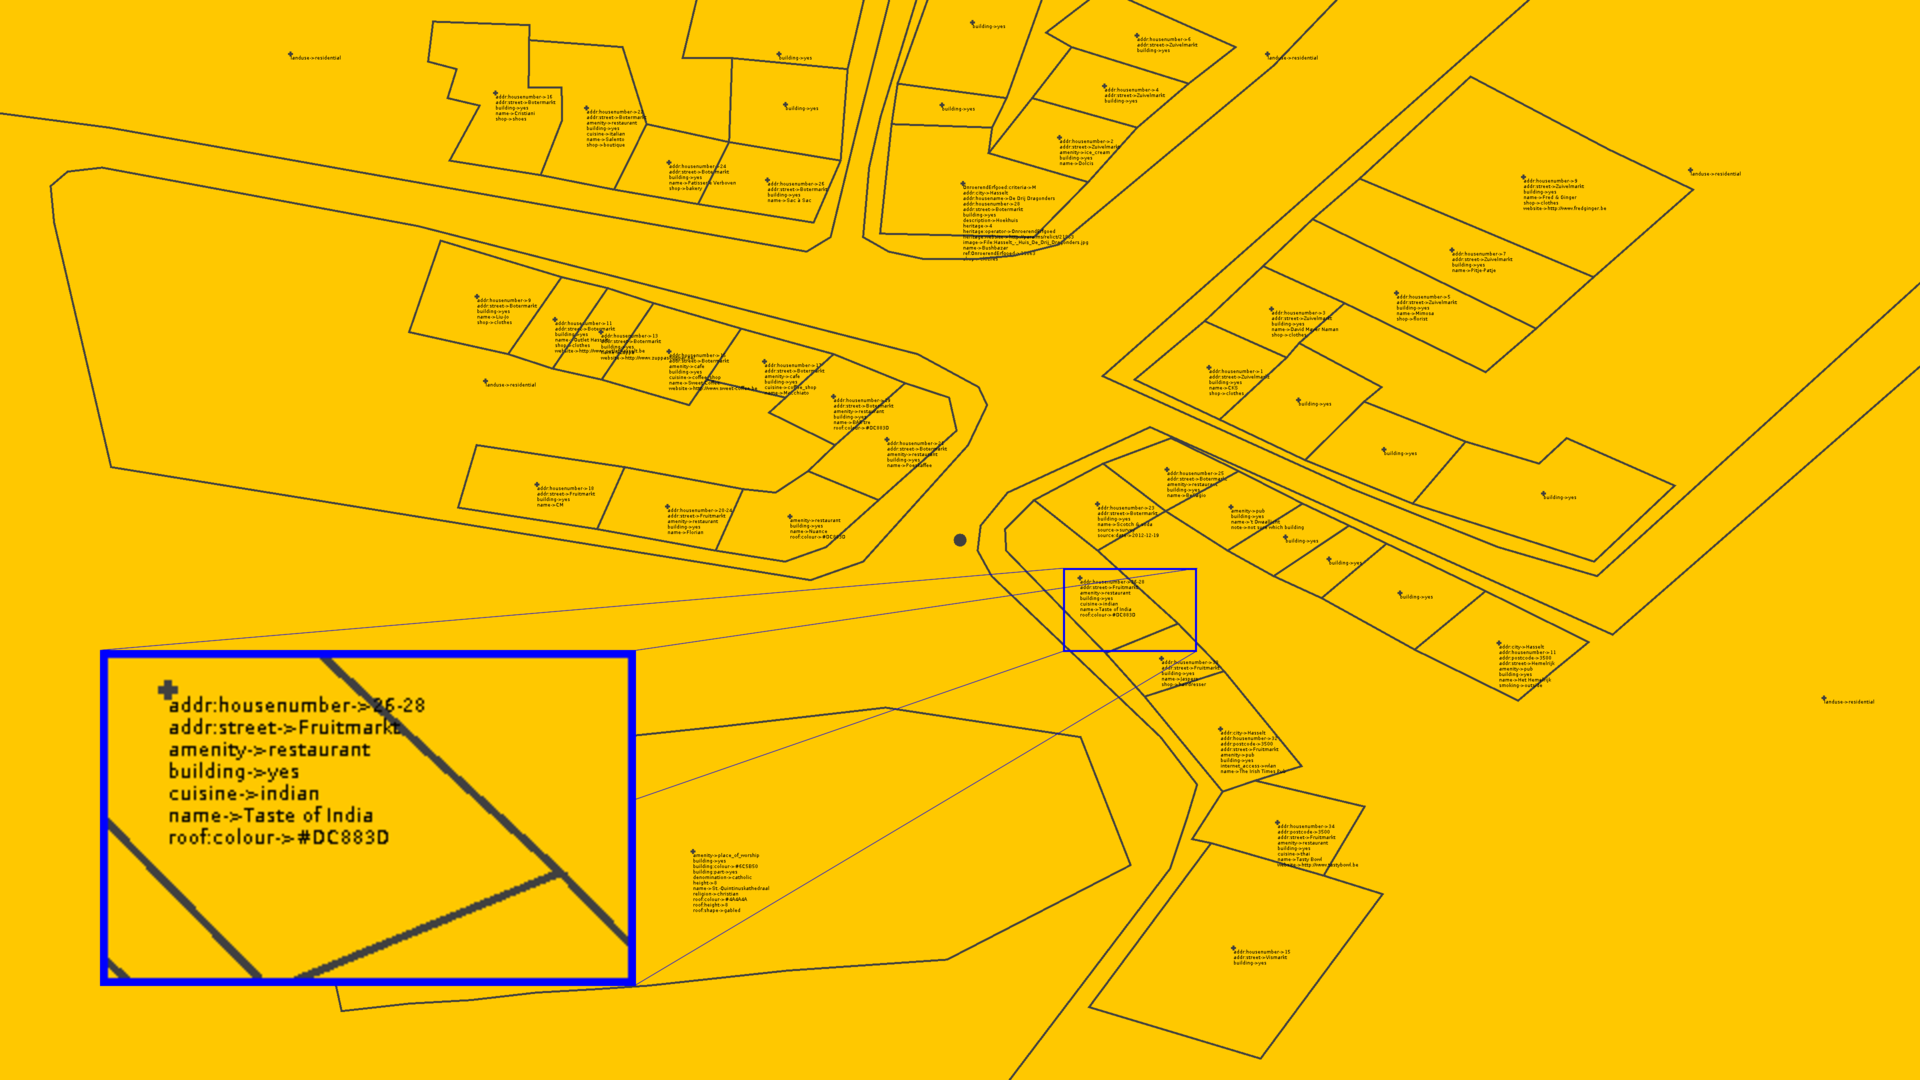
\includegraphics[width=\textwidth]{DataDrawer_raw_selected}}
\end{frame}

\begin{frame}
  \frametitle{Visualisierung}
  \Wider{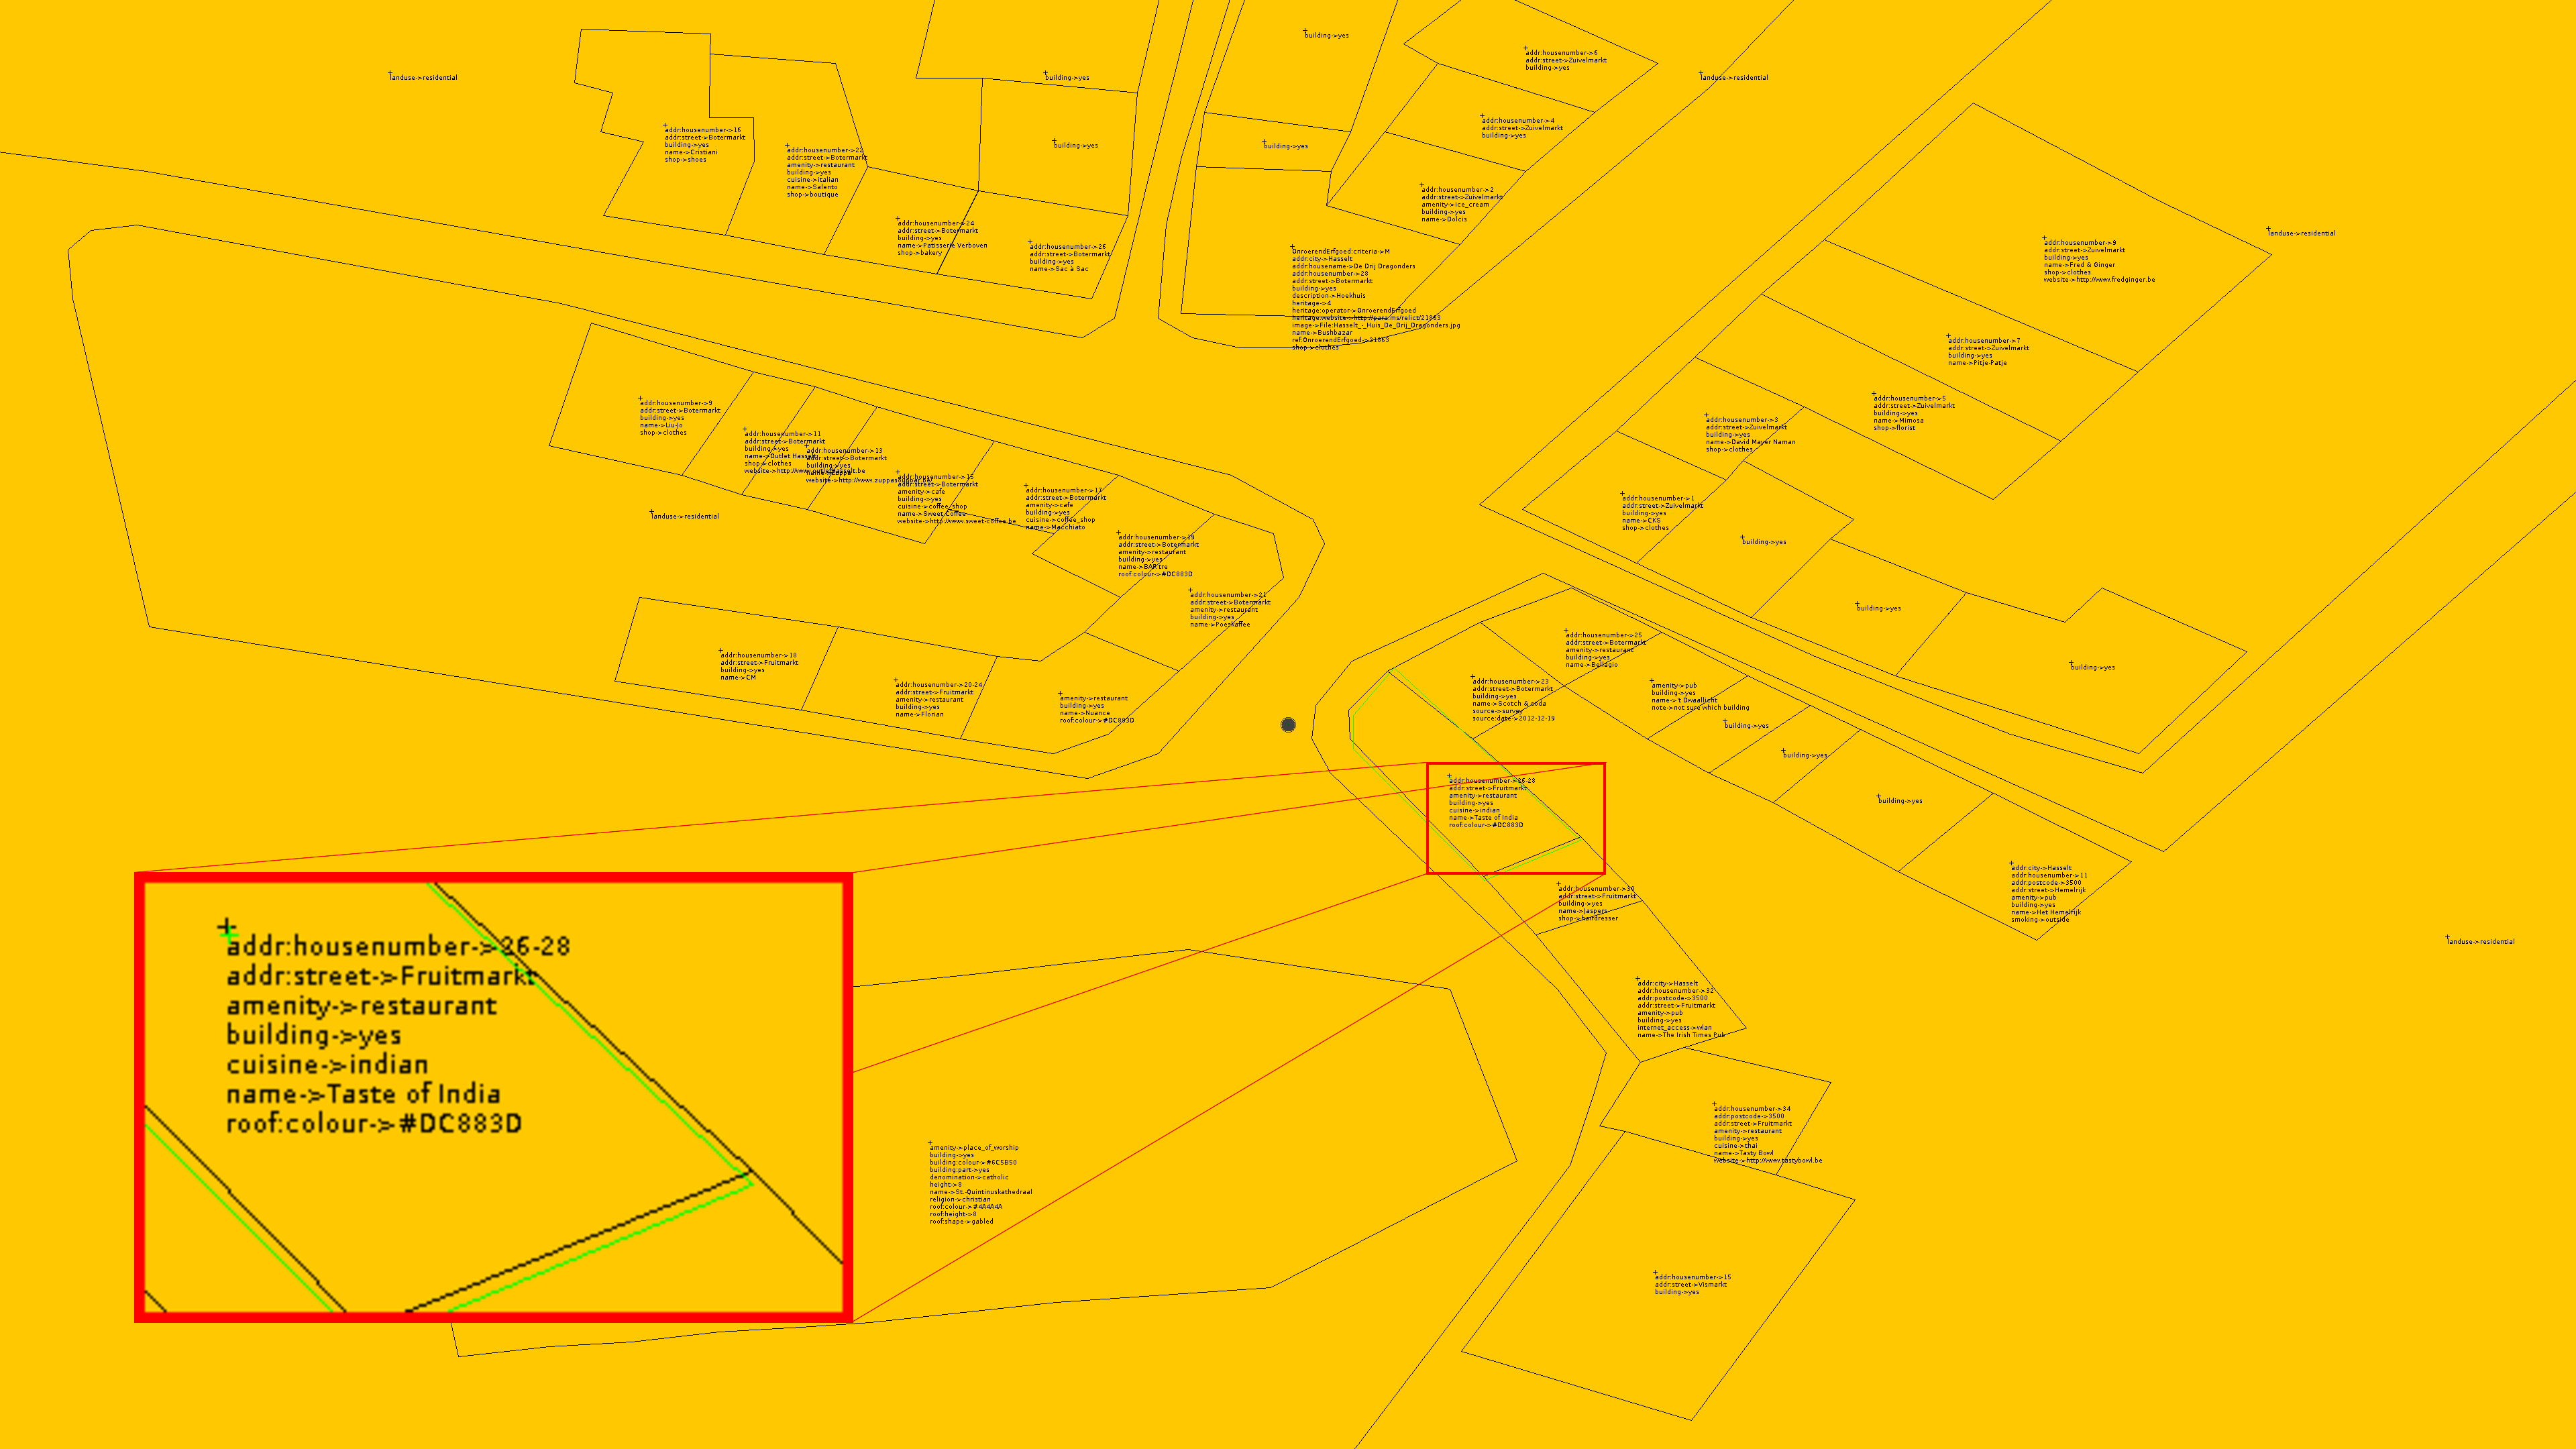
\includegraphics[width=\textwidth]{DataDrawer_truth_selected}}
\end{frame}

\begin{frame} %Distanzen ohne Gewichtung
 \frametitle{Grundidee}
  \Wider{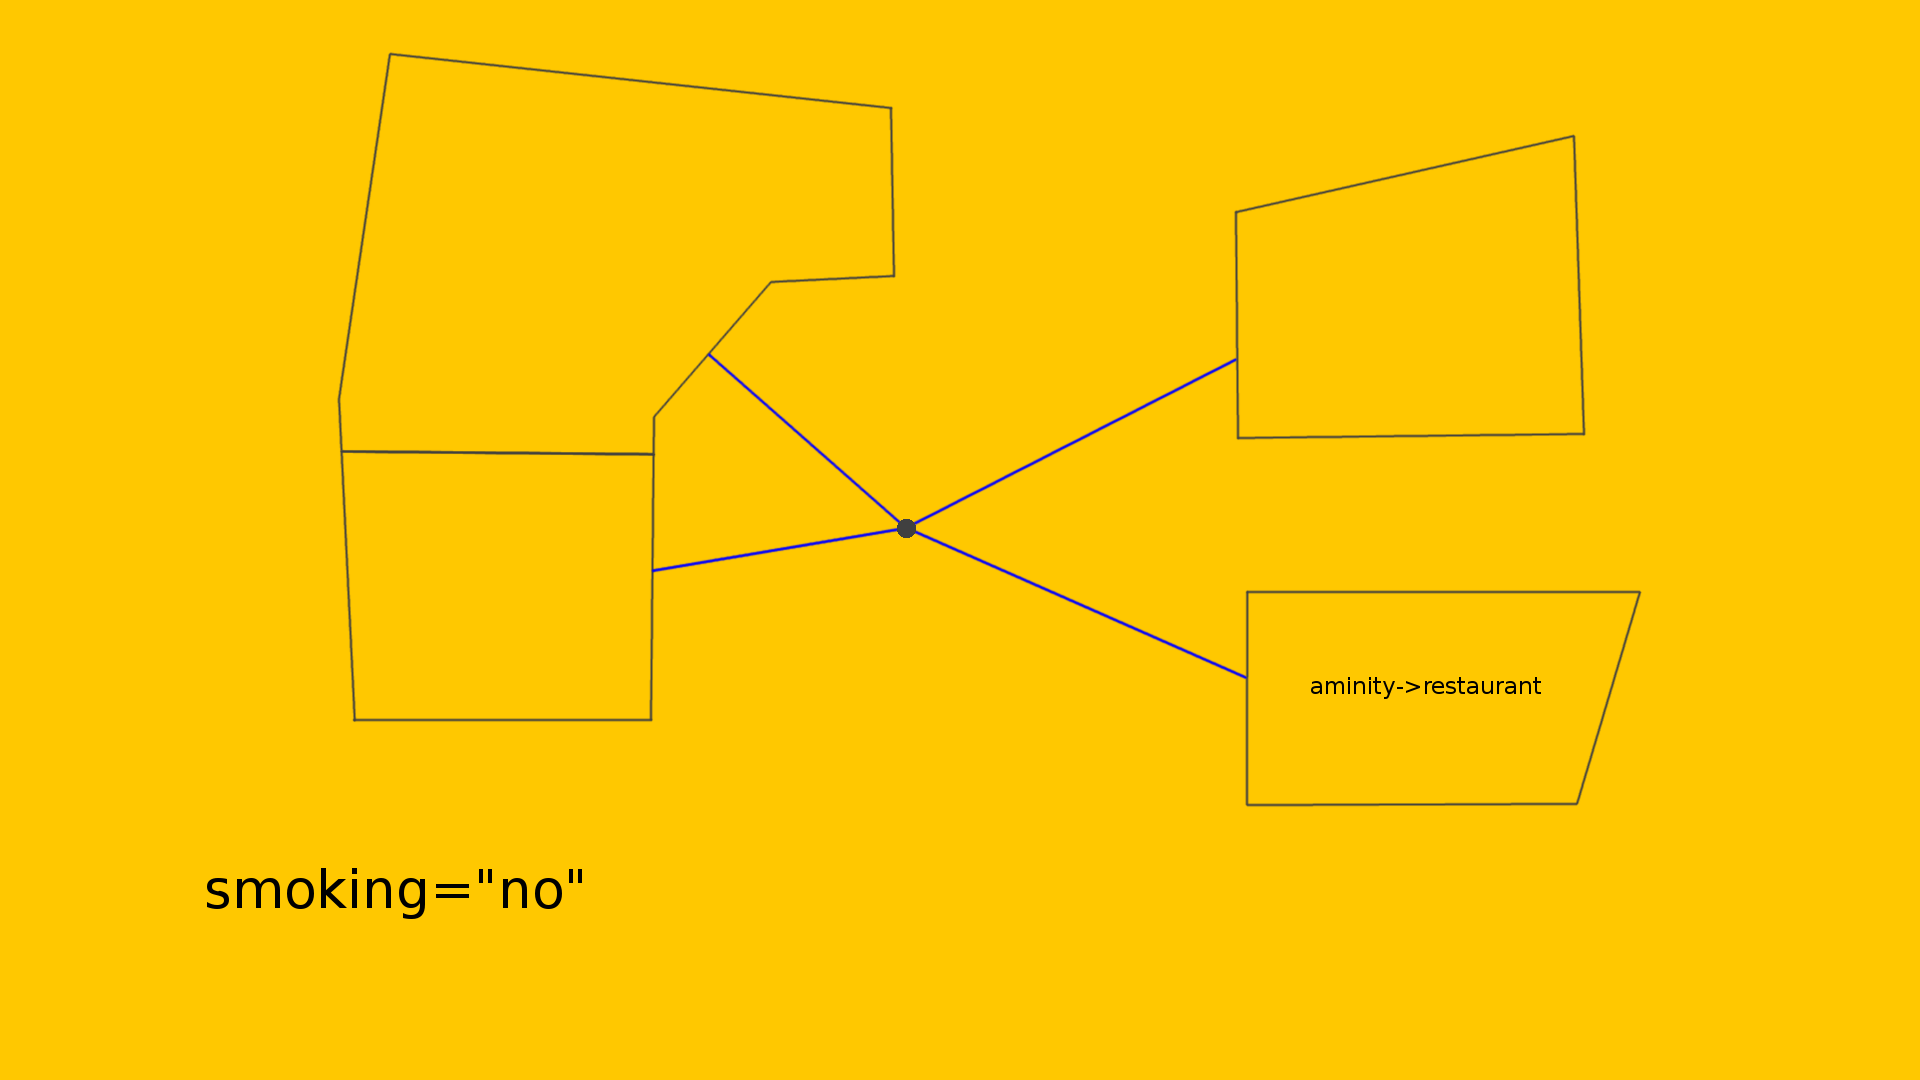
\includegraphics[width=\textwidth]{Funktionsweise_vorher}}
\end{frame}

\begin{frame} %Distanzen mit Gewichtung
 \frametitle{Grundidee}
  \Wider{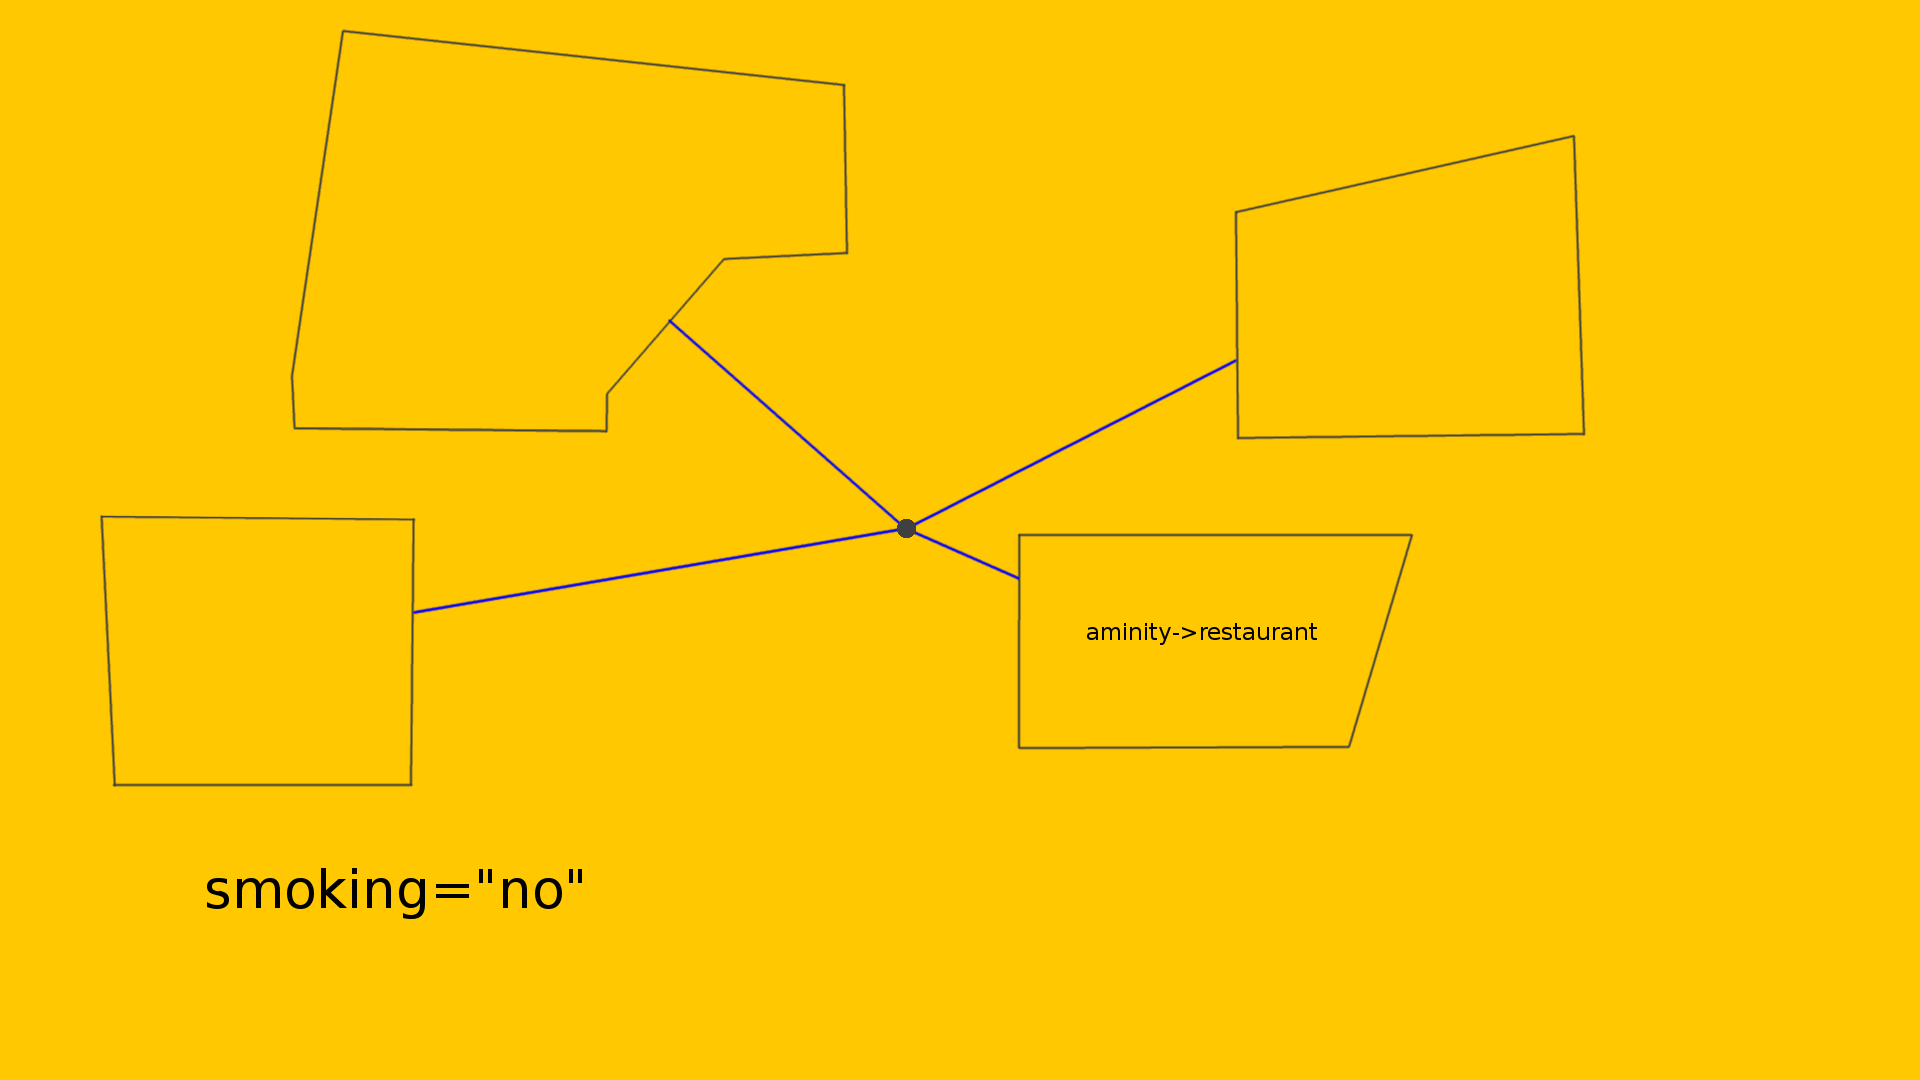
\includegraphics[width=\textwidth]{Funktionsweise_nachher}}
\end{frame}

\begin{frame}
  \frametitle{Formel}
  \begin{Large}
  \begin{equation*}
    dist_{new} = (offset + dist_{old}) \prod_{t\in P} w_{t}
  \end{equation*}
  \qquad \\
\begin{equation*}
\begin{array}{r l}
 P & \text{eine Fl\"ache in OSM},\\
 t & \text{Tag der Fl\"ache }P,\\
 w_t & \text{Gewicht des Tags $t$}.
\end{array}
\end{equation*}
\end{Large}
\end{frame}

\begin{frame}
  \frametitle{Visualisierung}
  \Wider{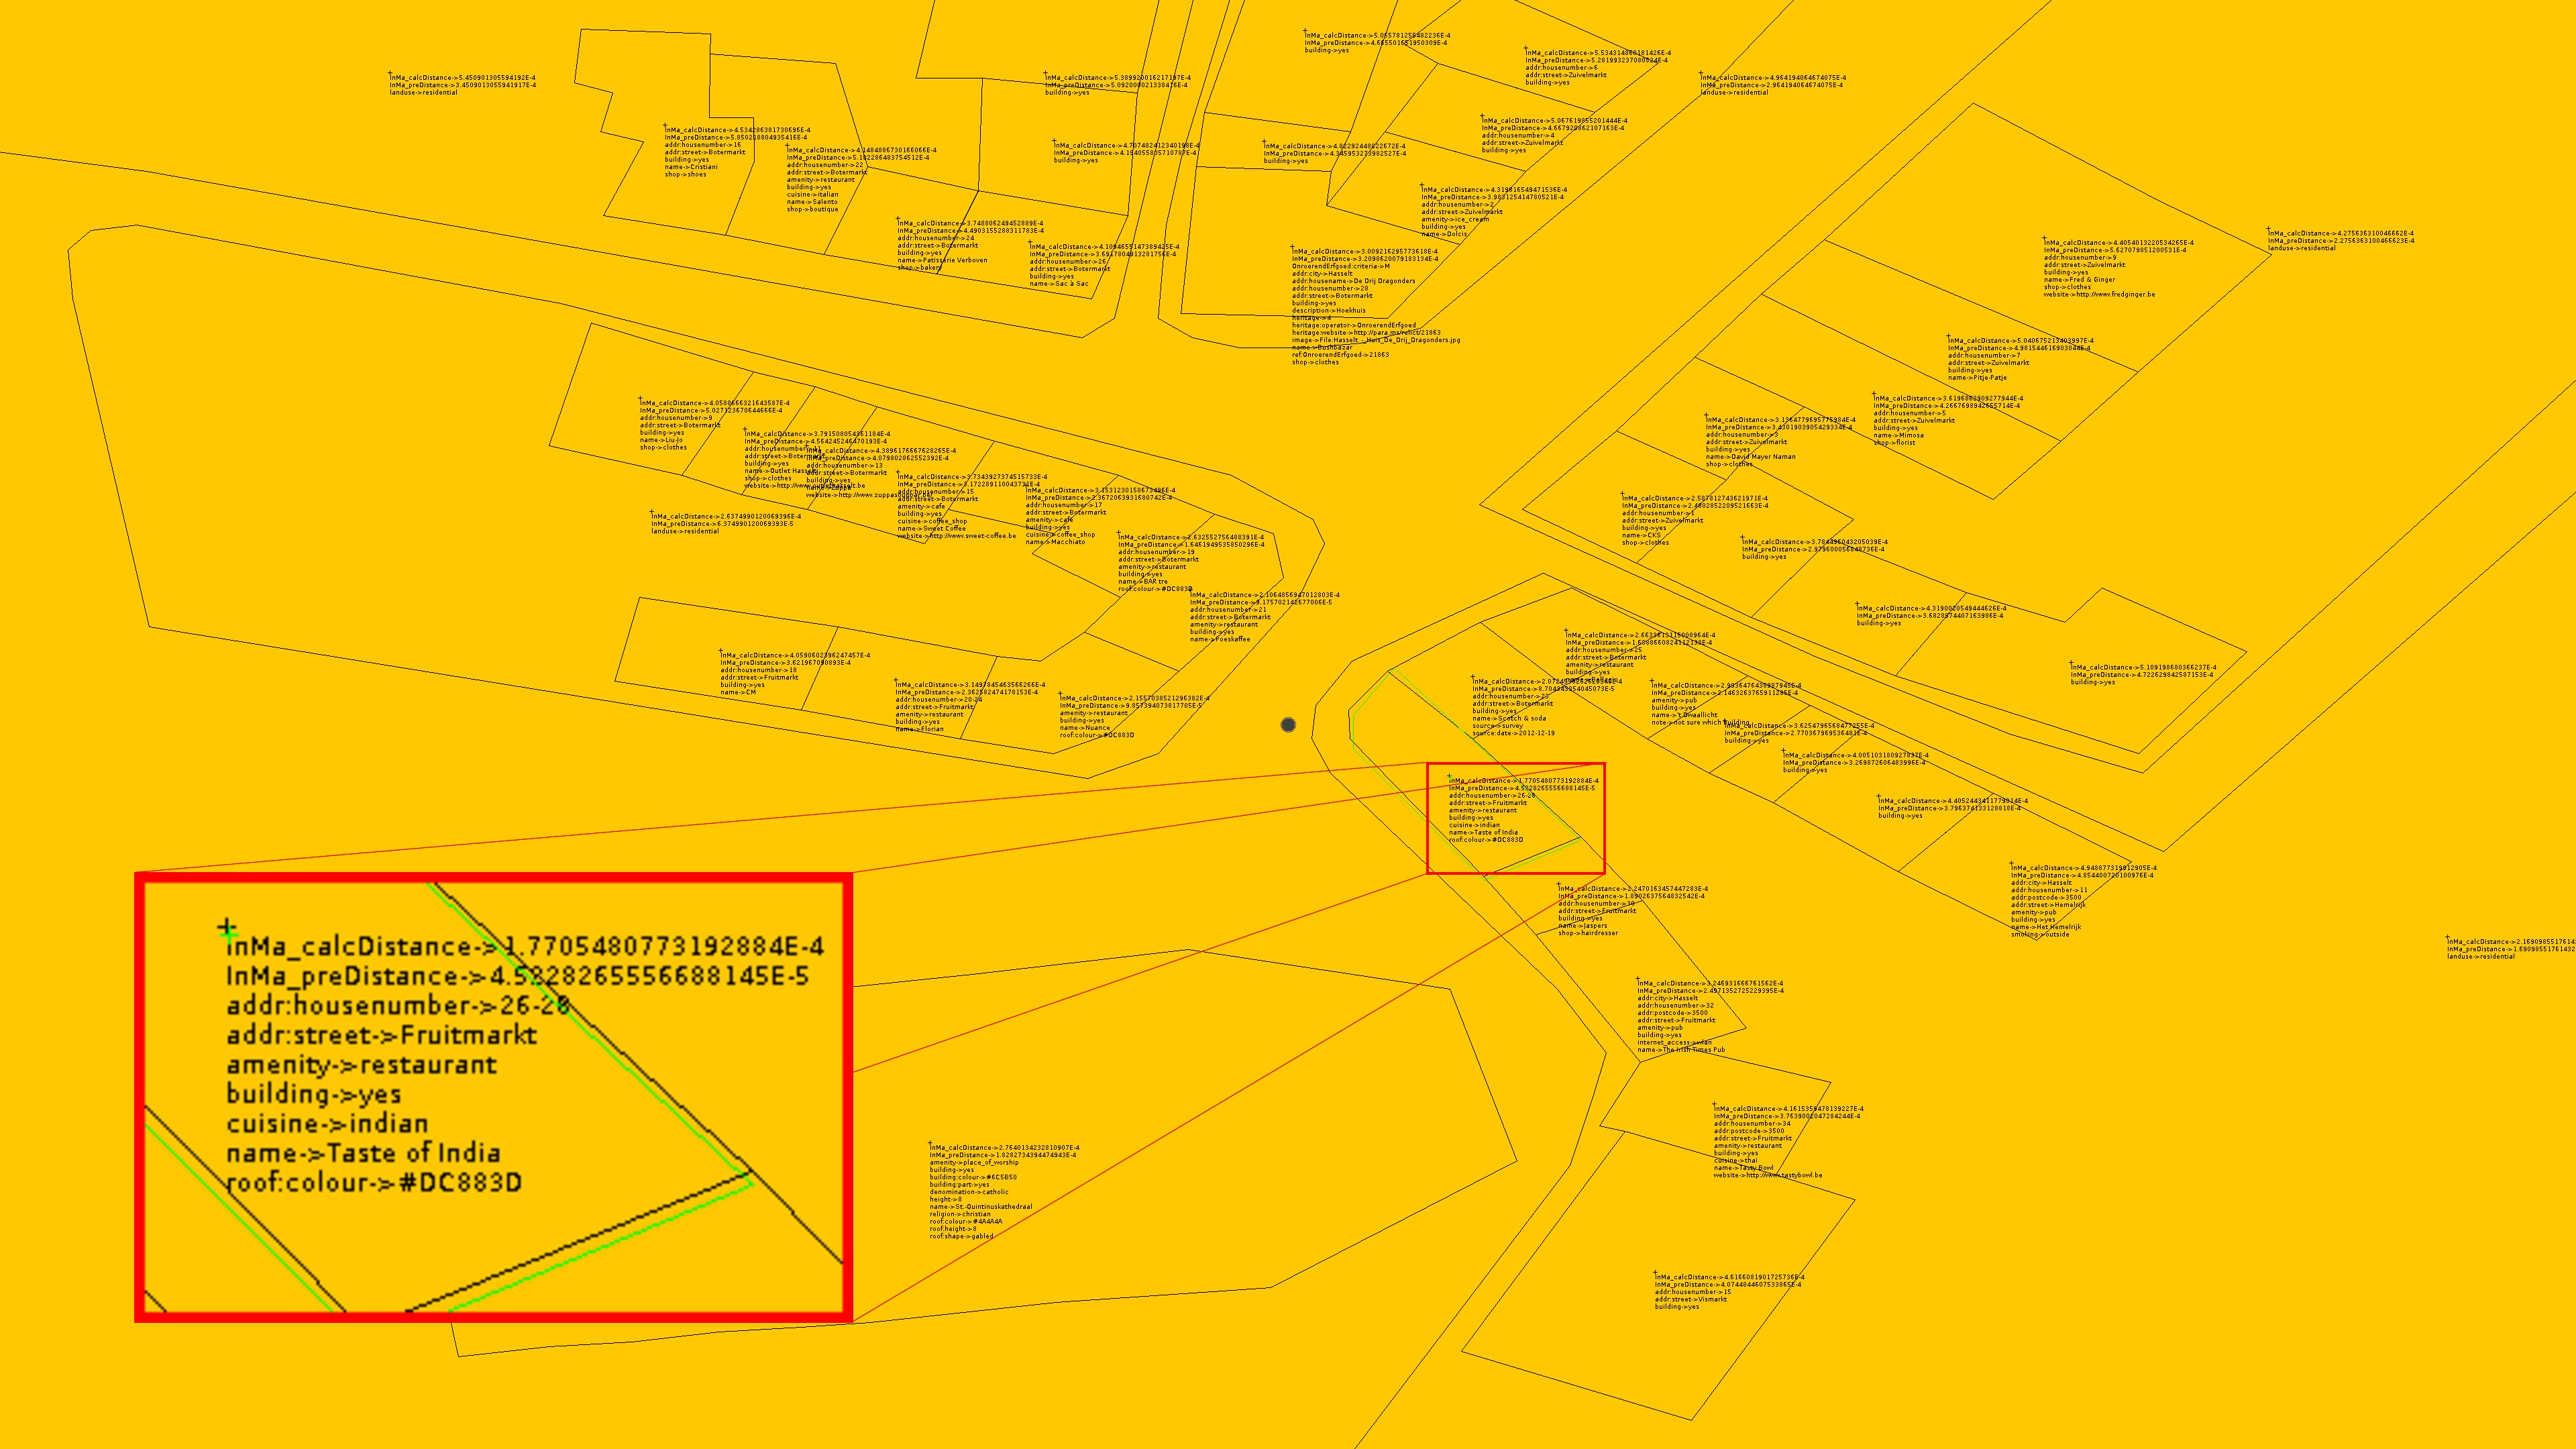
\includegraphics[width=\textwidth]{DataDrawer_dist_selected}}
\end{frame}

\begin{frame}
  \frametitle{Visualisierung}
  \Wider{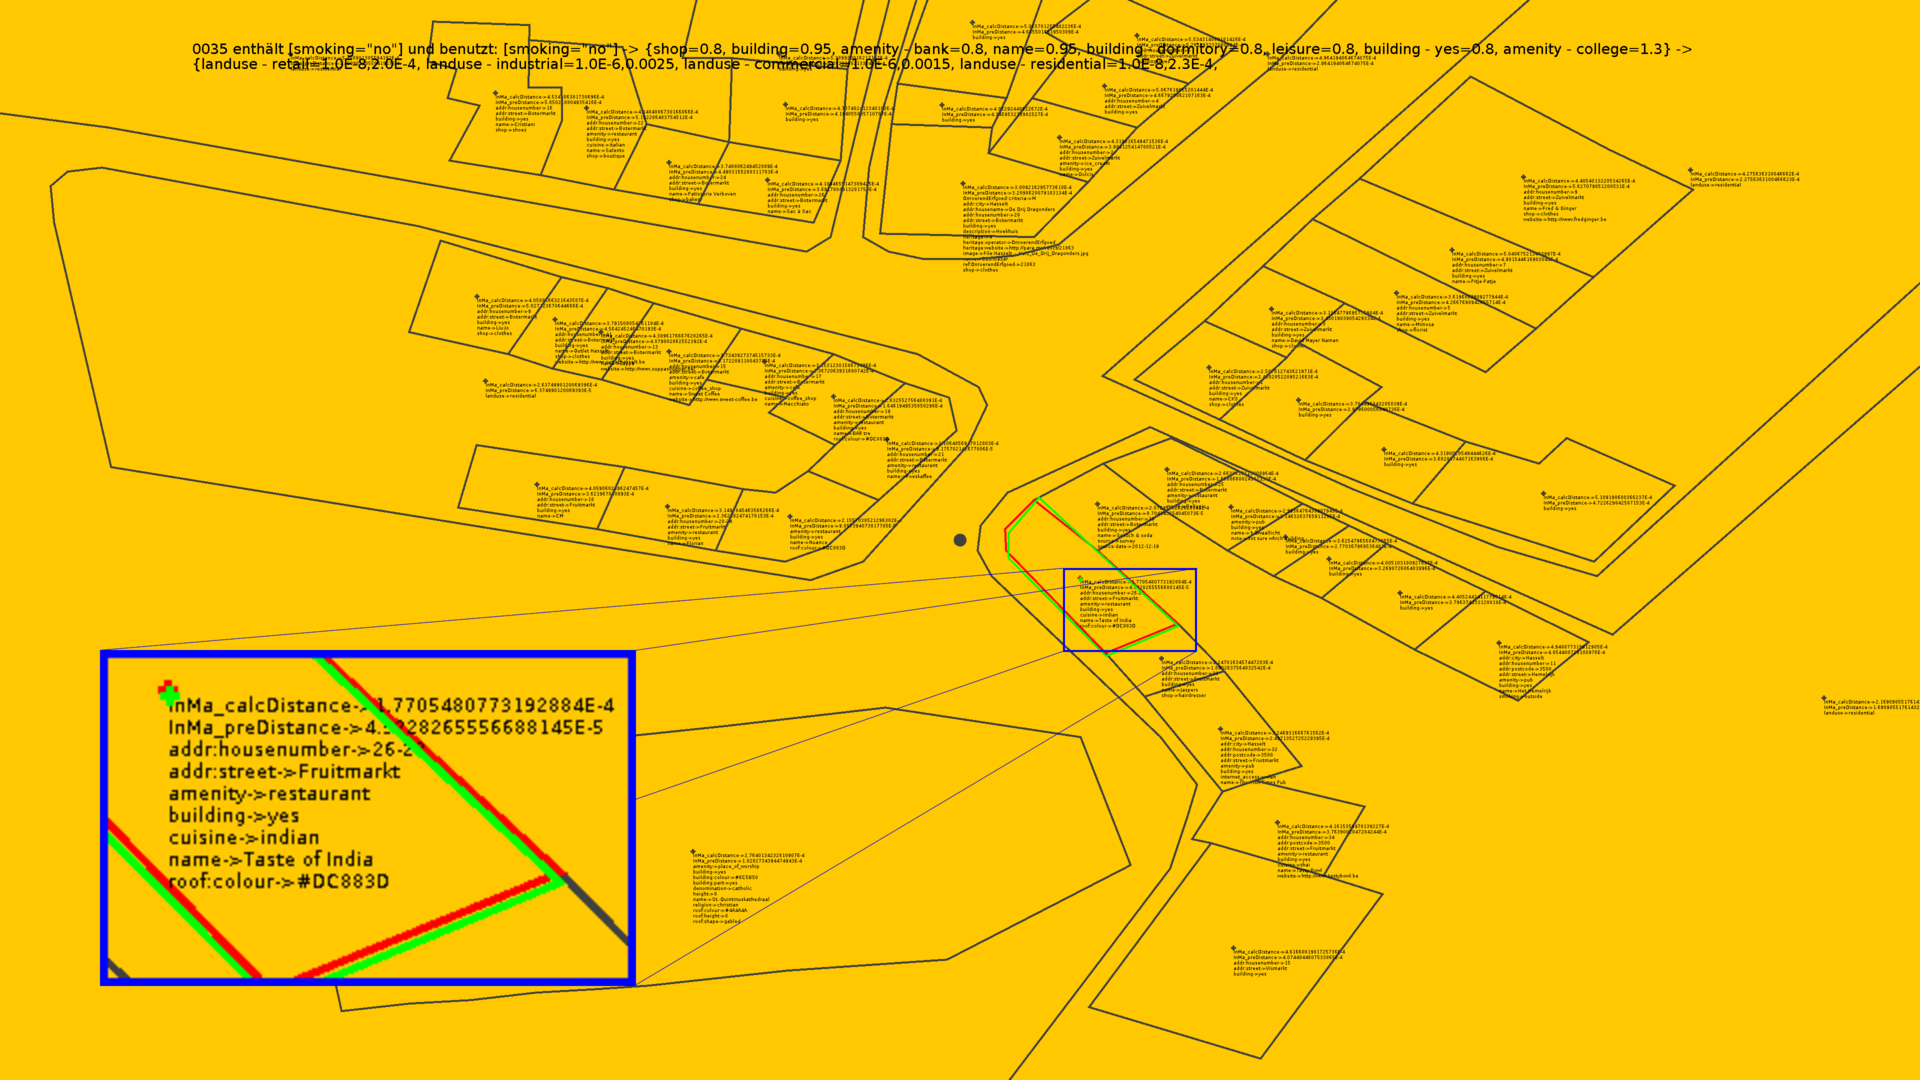
\includegraphics[width=\textwidth]{DataDrawer_rules_selected}}
\end{frame}

%%\begin{frame}
%  \frametitle{Visualisierung}
%  \Wider{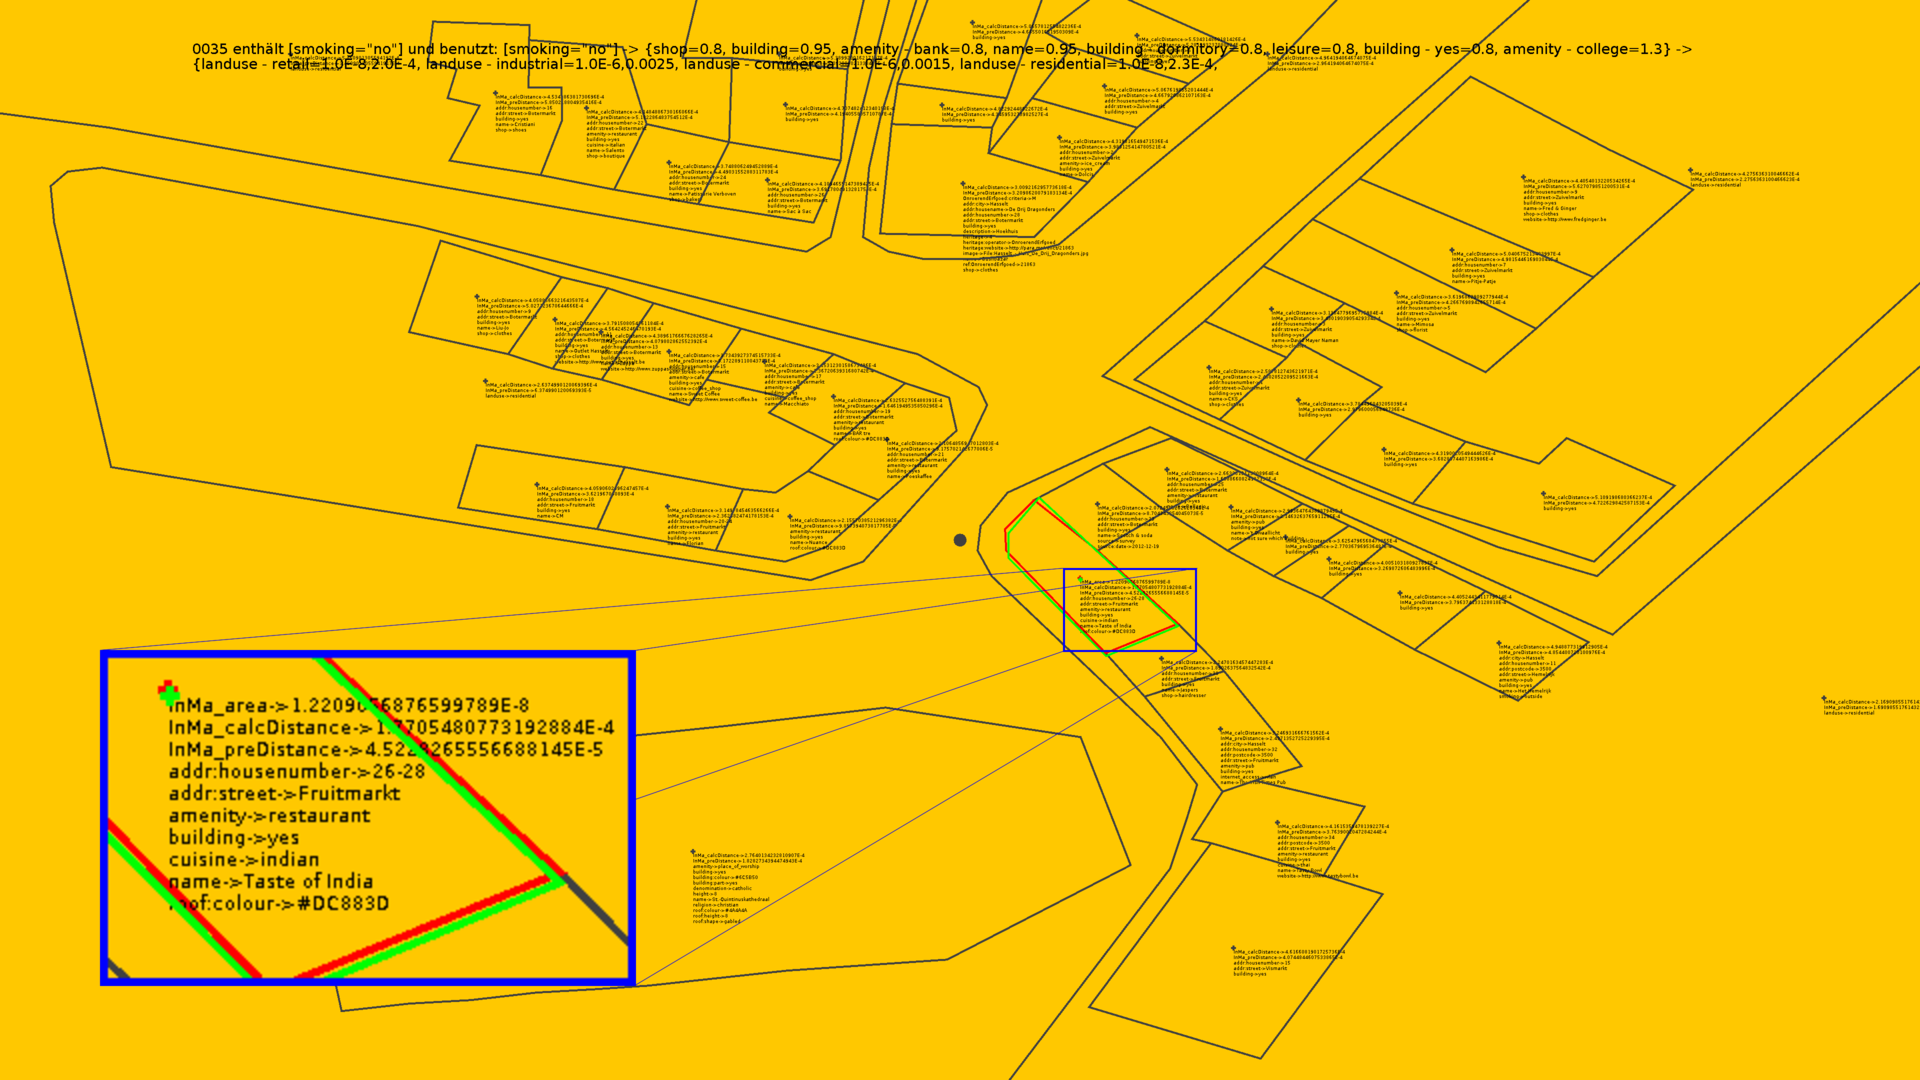
\includegraphics[width=\textwidth]{DataDrawer_area_selected}}
%\end{frame}

\begin{frame}
  \frametitle{Coverage}
  \begin{equation*}
    Coverage = \frac{Area_{intersection}}{max(Area_{guesspolygon},Area_{loesungspolygon})}
  \end{equation*}
\\
  \begin{equation*}
    Coverage \in {0..1}
  \end{equation*}
%%%%%%%%%%%%%%%%%%%%%%%%%%%%%%%%%%%%%%%%%%%%%%%%%%%%%%%%%%%%%%%%%%%%%%%%%%%%%%%%
% Vielleicht hier 3 kleine Beispiele für Coverage.
% 0: intersection = null
% 1: intersection = lösung  % oder beliebige andere
% 0.1: Lösung ist 1/10 von guess groß und liegt in ihr drinne
%%%%%%%%%%%%%%%%%%%%%%%%%%%%%%%%%%%%%%%%%%%%%%%%%%%%%%%%%%%%%%%%%%%%%%%%%%%%%%%%
\end{frame}

\begin{frame}
  \frametitle{Naiver Ansatz}
  \begin{center}
  \huge{Coverage = 49,6 \%}
  \end{center}
\end{frame}

\begin{frame}
  \frametitle{Gewichteter Ansatz}
  \begin{center}
  \huge{Coverage = 69,8 \%}
  \end{center}
  \begin{center}
  Naive Coverage = 49,6 \%
  \end{center}
\end{frame}


\begin{frame}
  \frametitle{Unvollständige Datensätze \hfill Nr. 38}
  \Wider{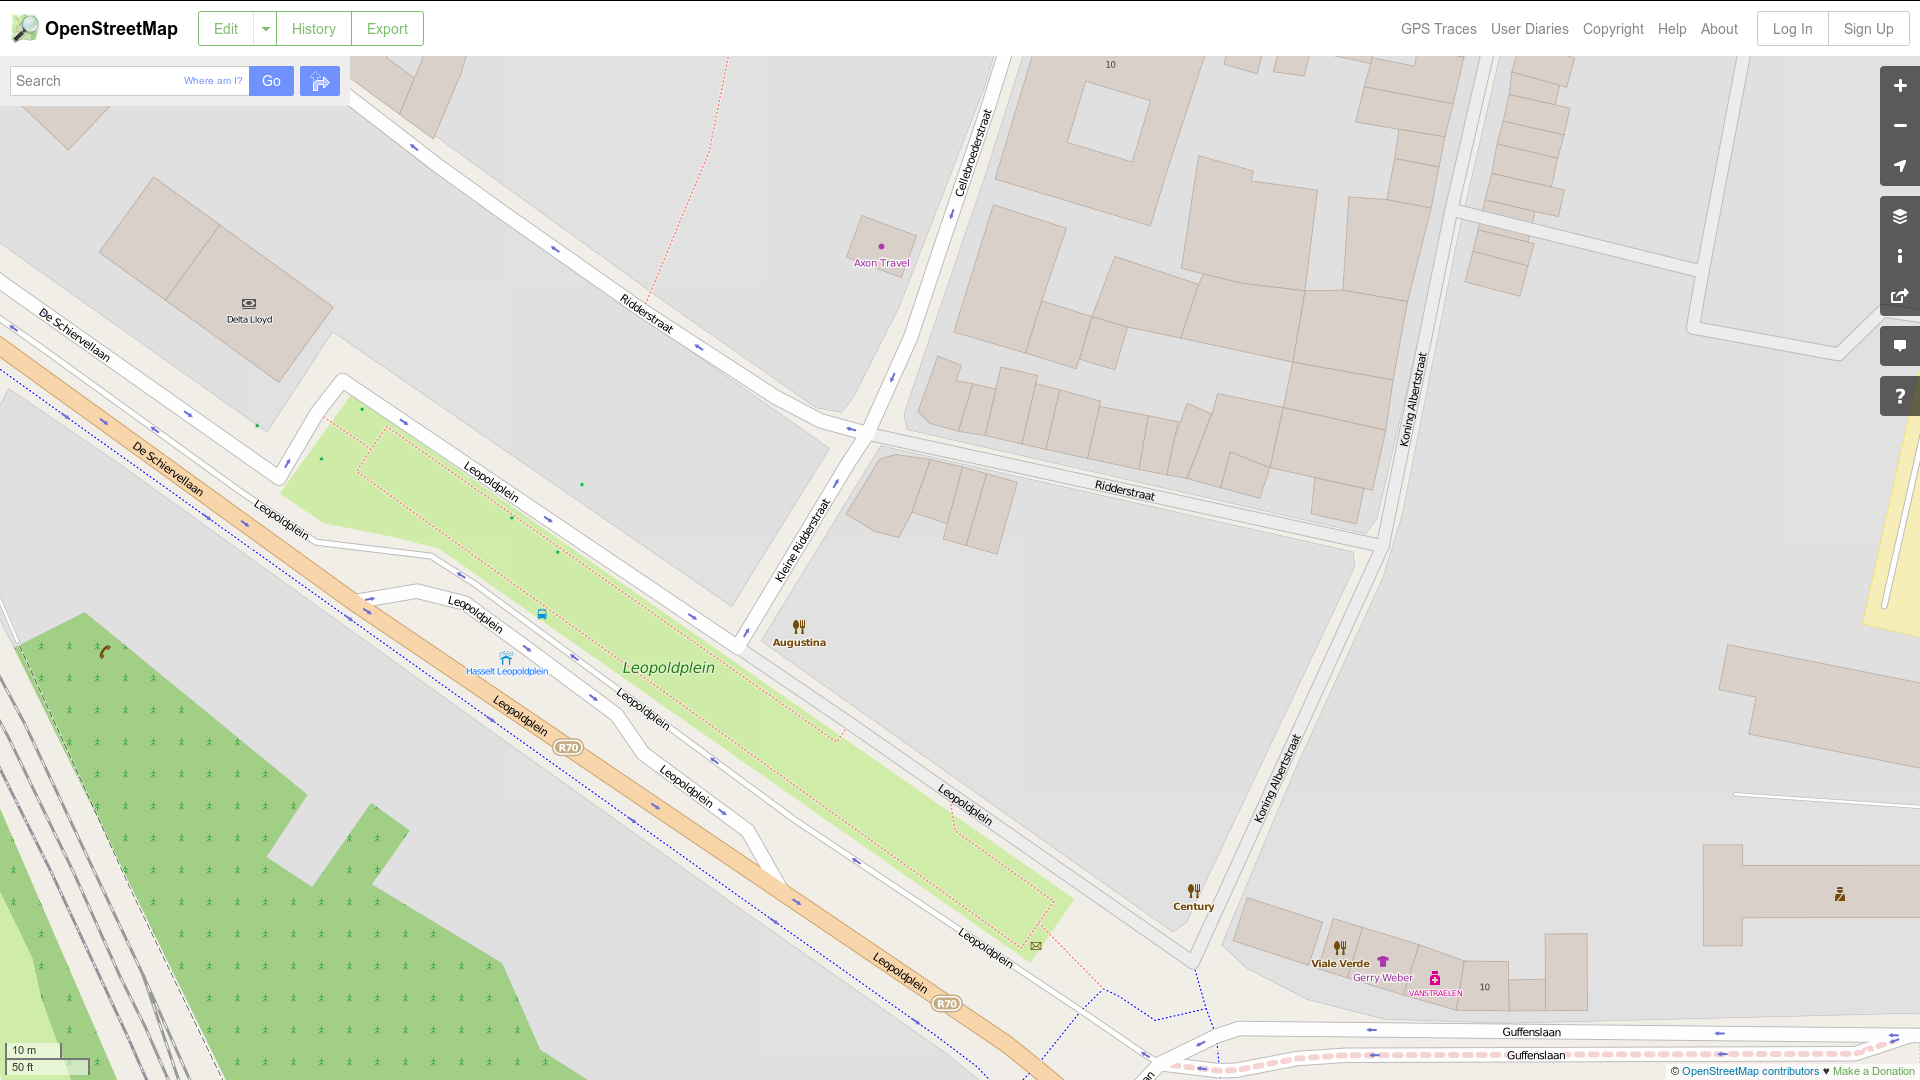
\includegraphics[width=\textwidth]{unvollstaendig}}
\end{frame}


\begin{frame}
  \frametitle{Unvollständige Datensätze \hfill Nr. 38}
  \Wider{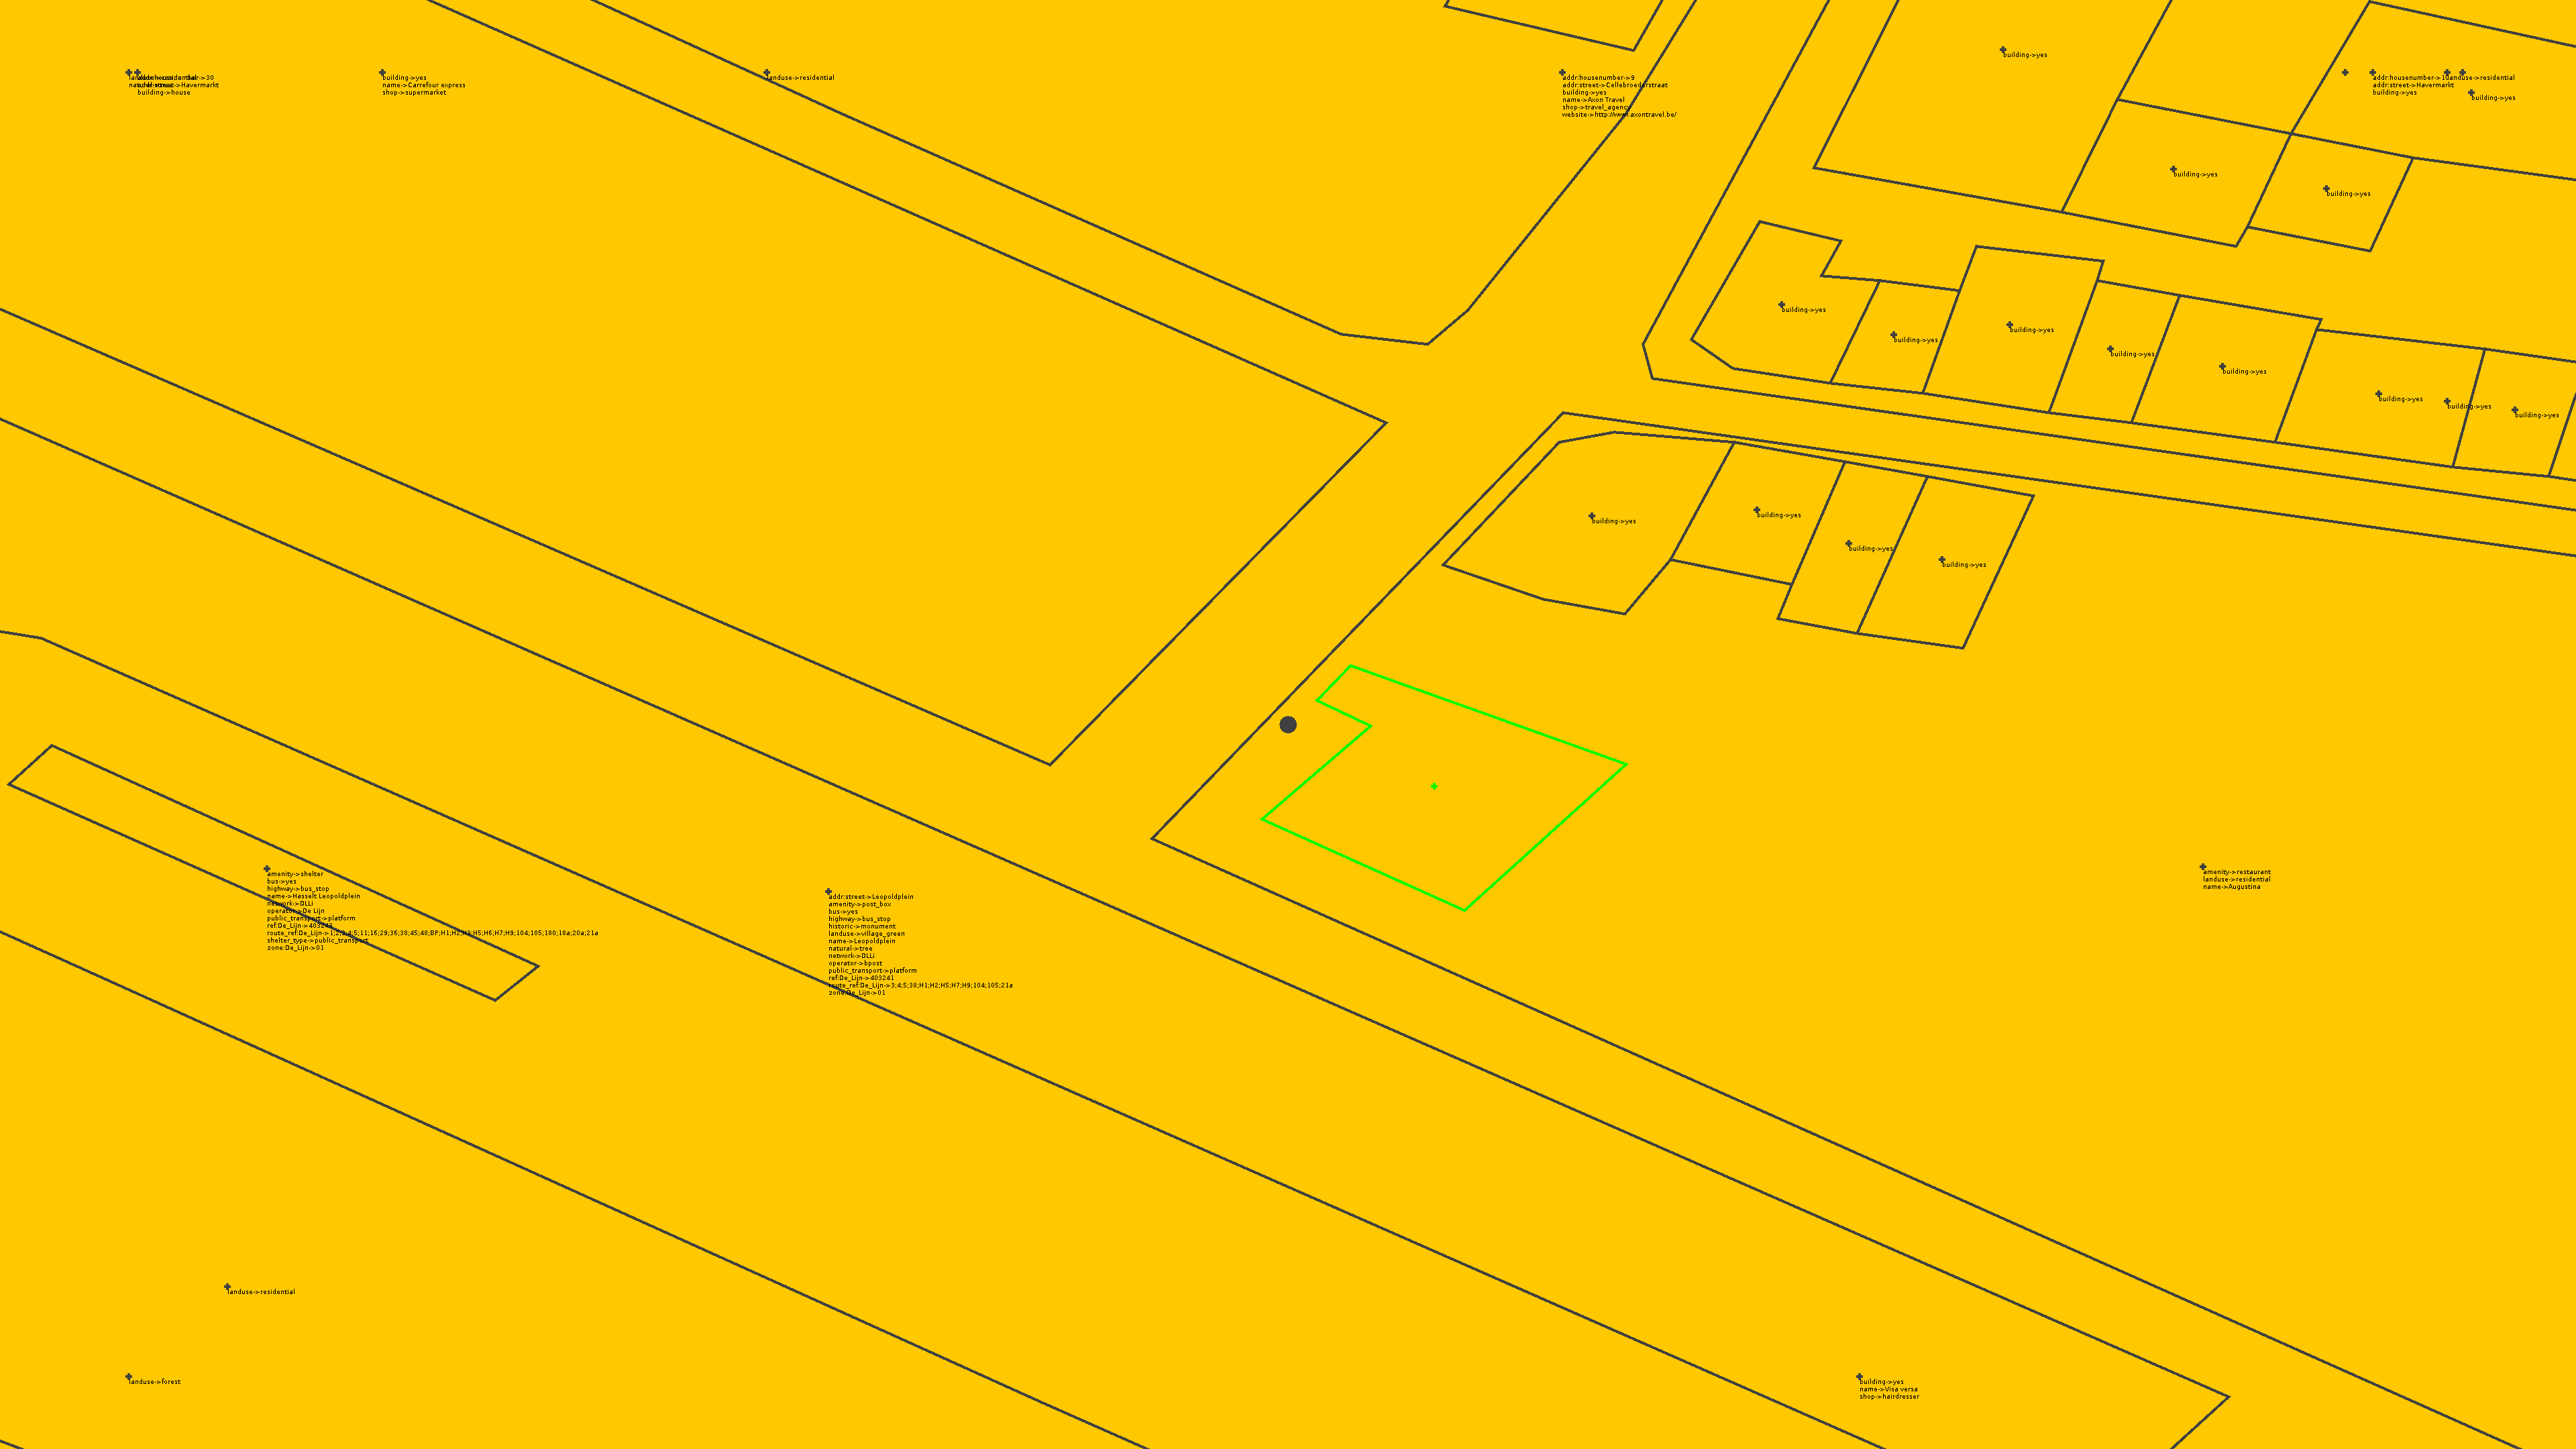
\includegraphics[width=\textwidth]{unvoll_ours}}
\end{frame}


\begin{frame}
  \frametitle{Unvollständige Datensätze \hfill Nr. 38}
  \Wider{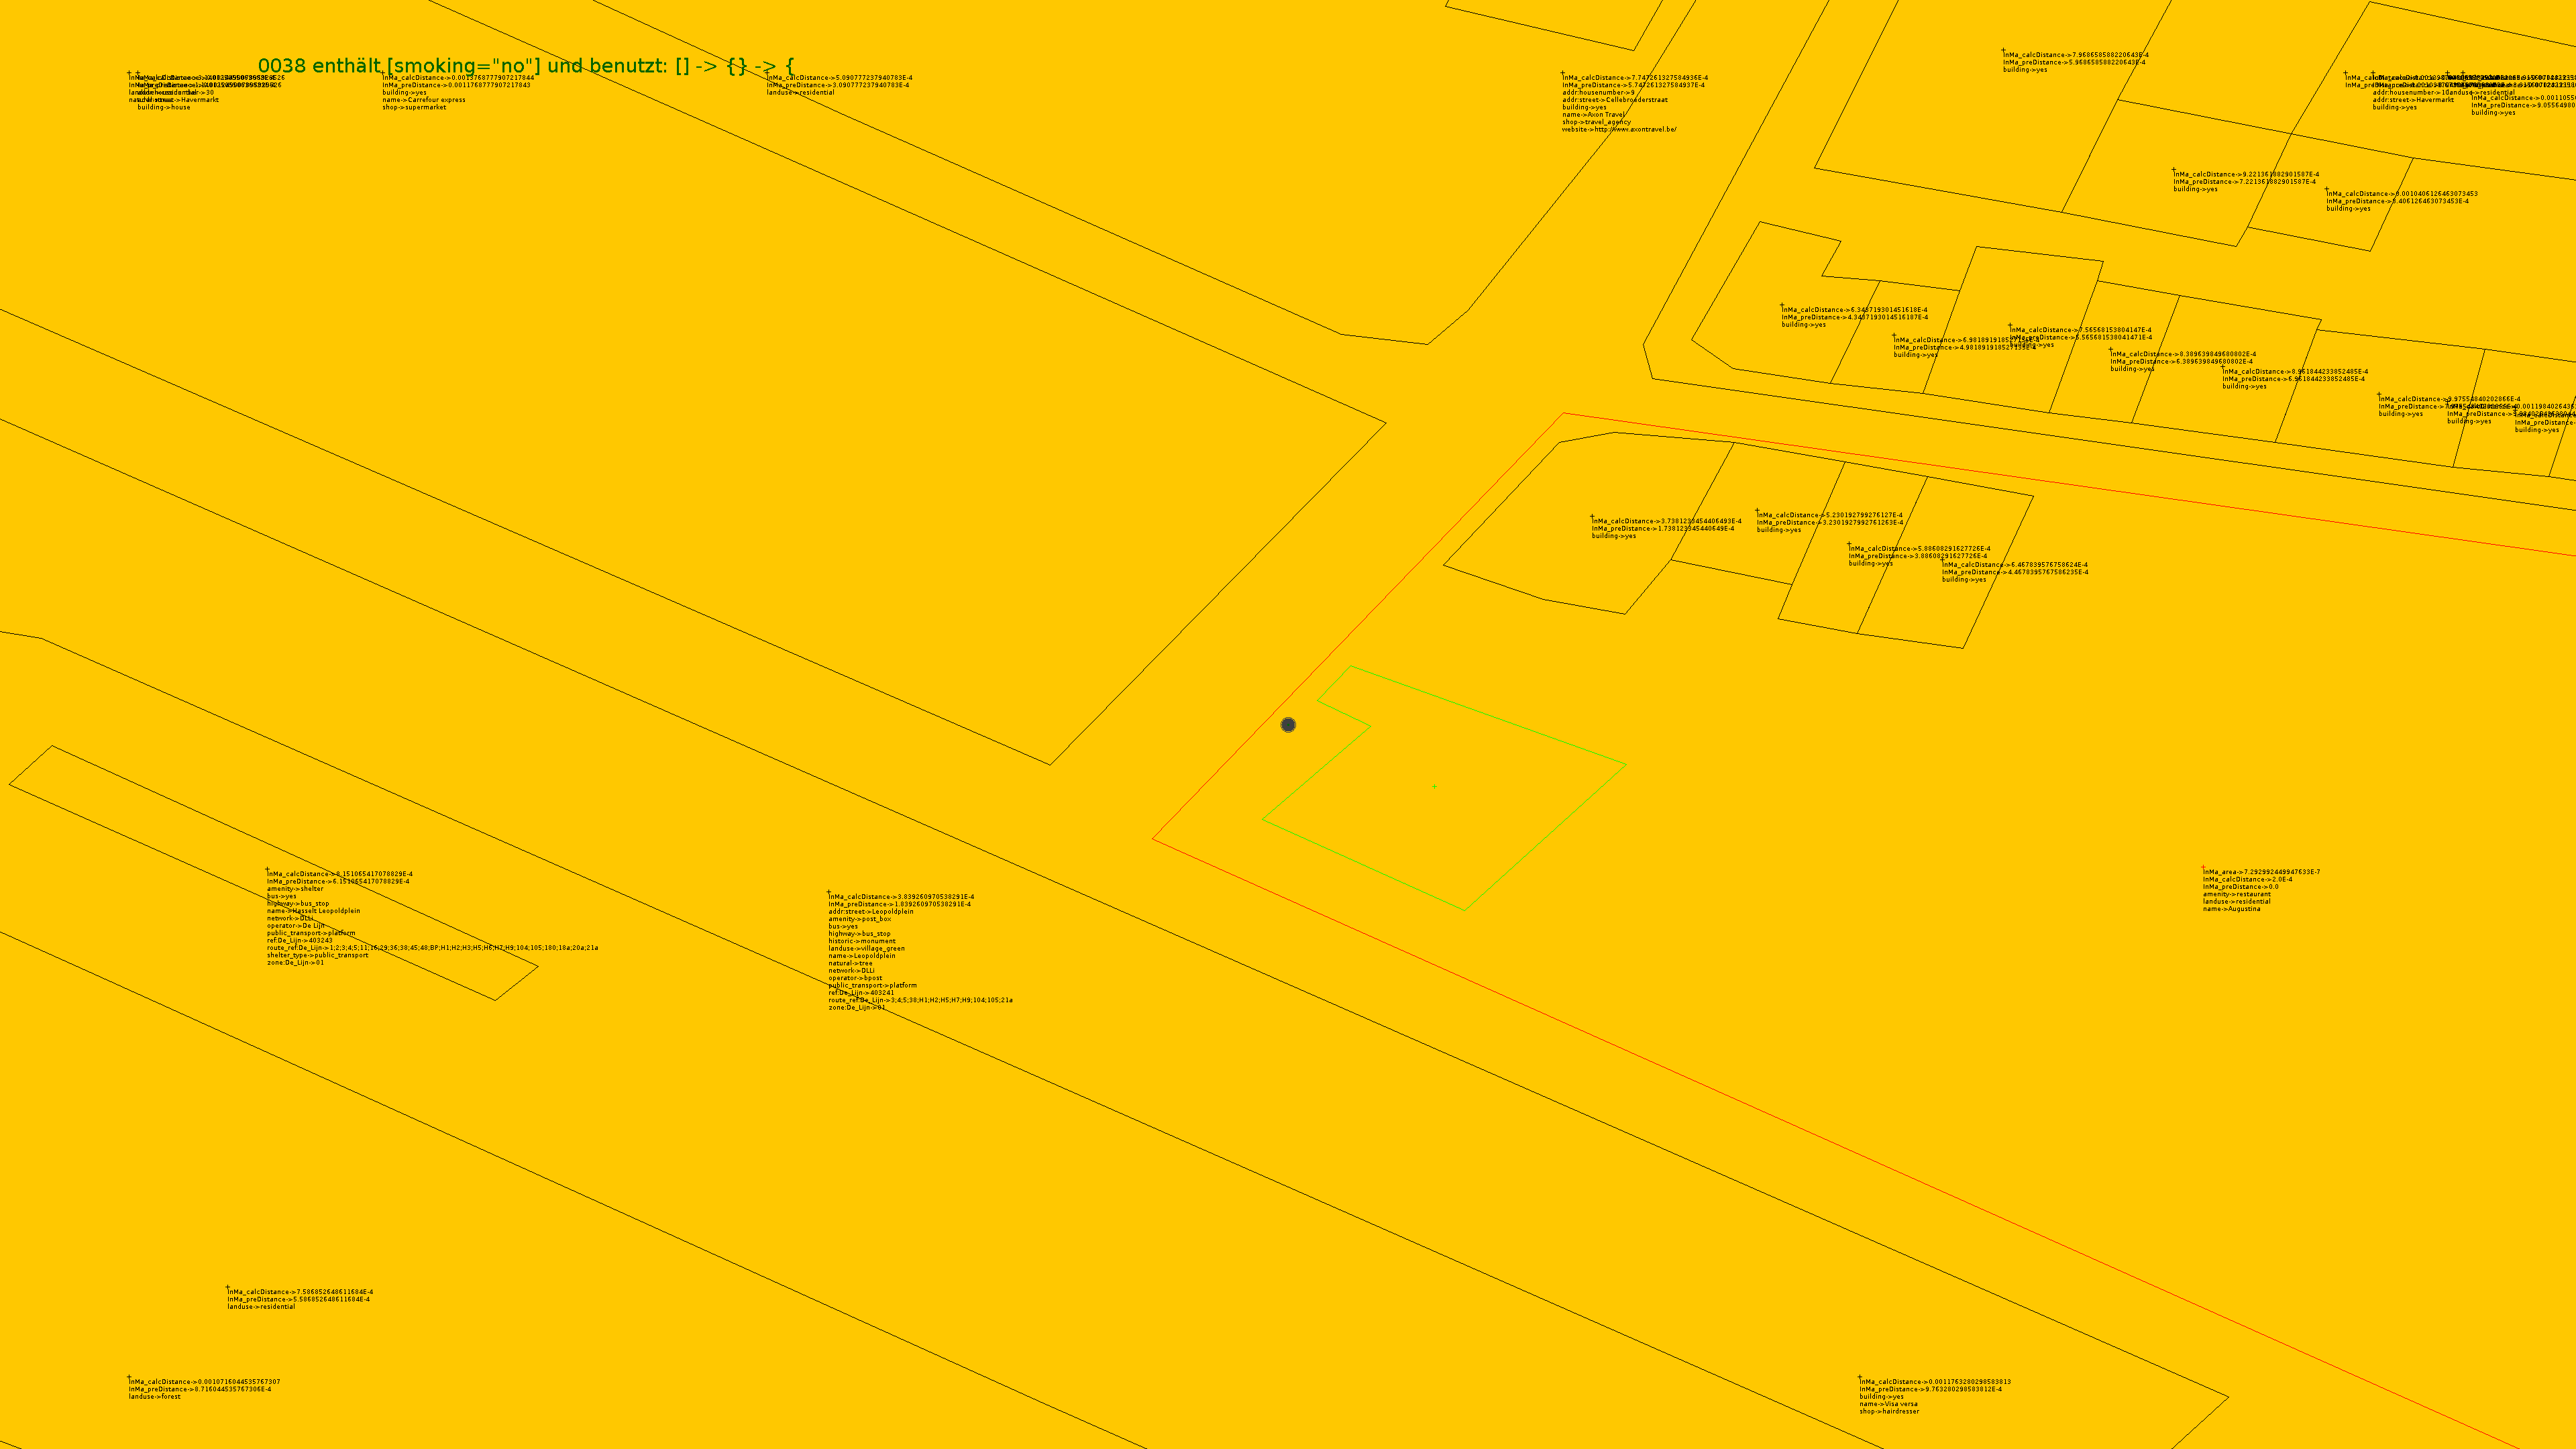
\includegraphics[width=\textwidth]{unvoll_naive}}
\end{frame}


\begin{frame}
  \frametitle{Umgebungspolygon}
  \Wider{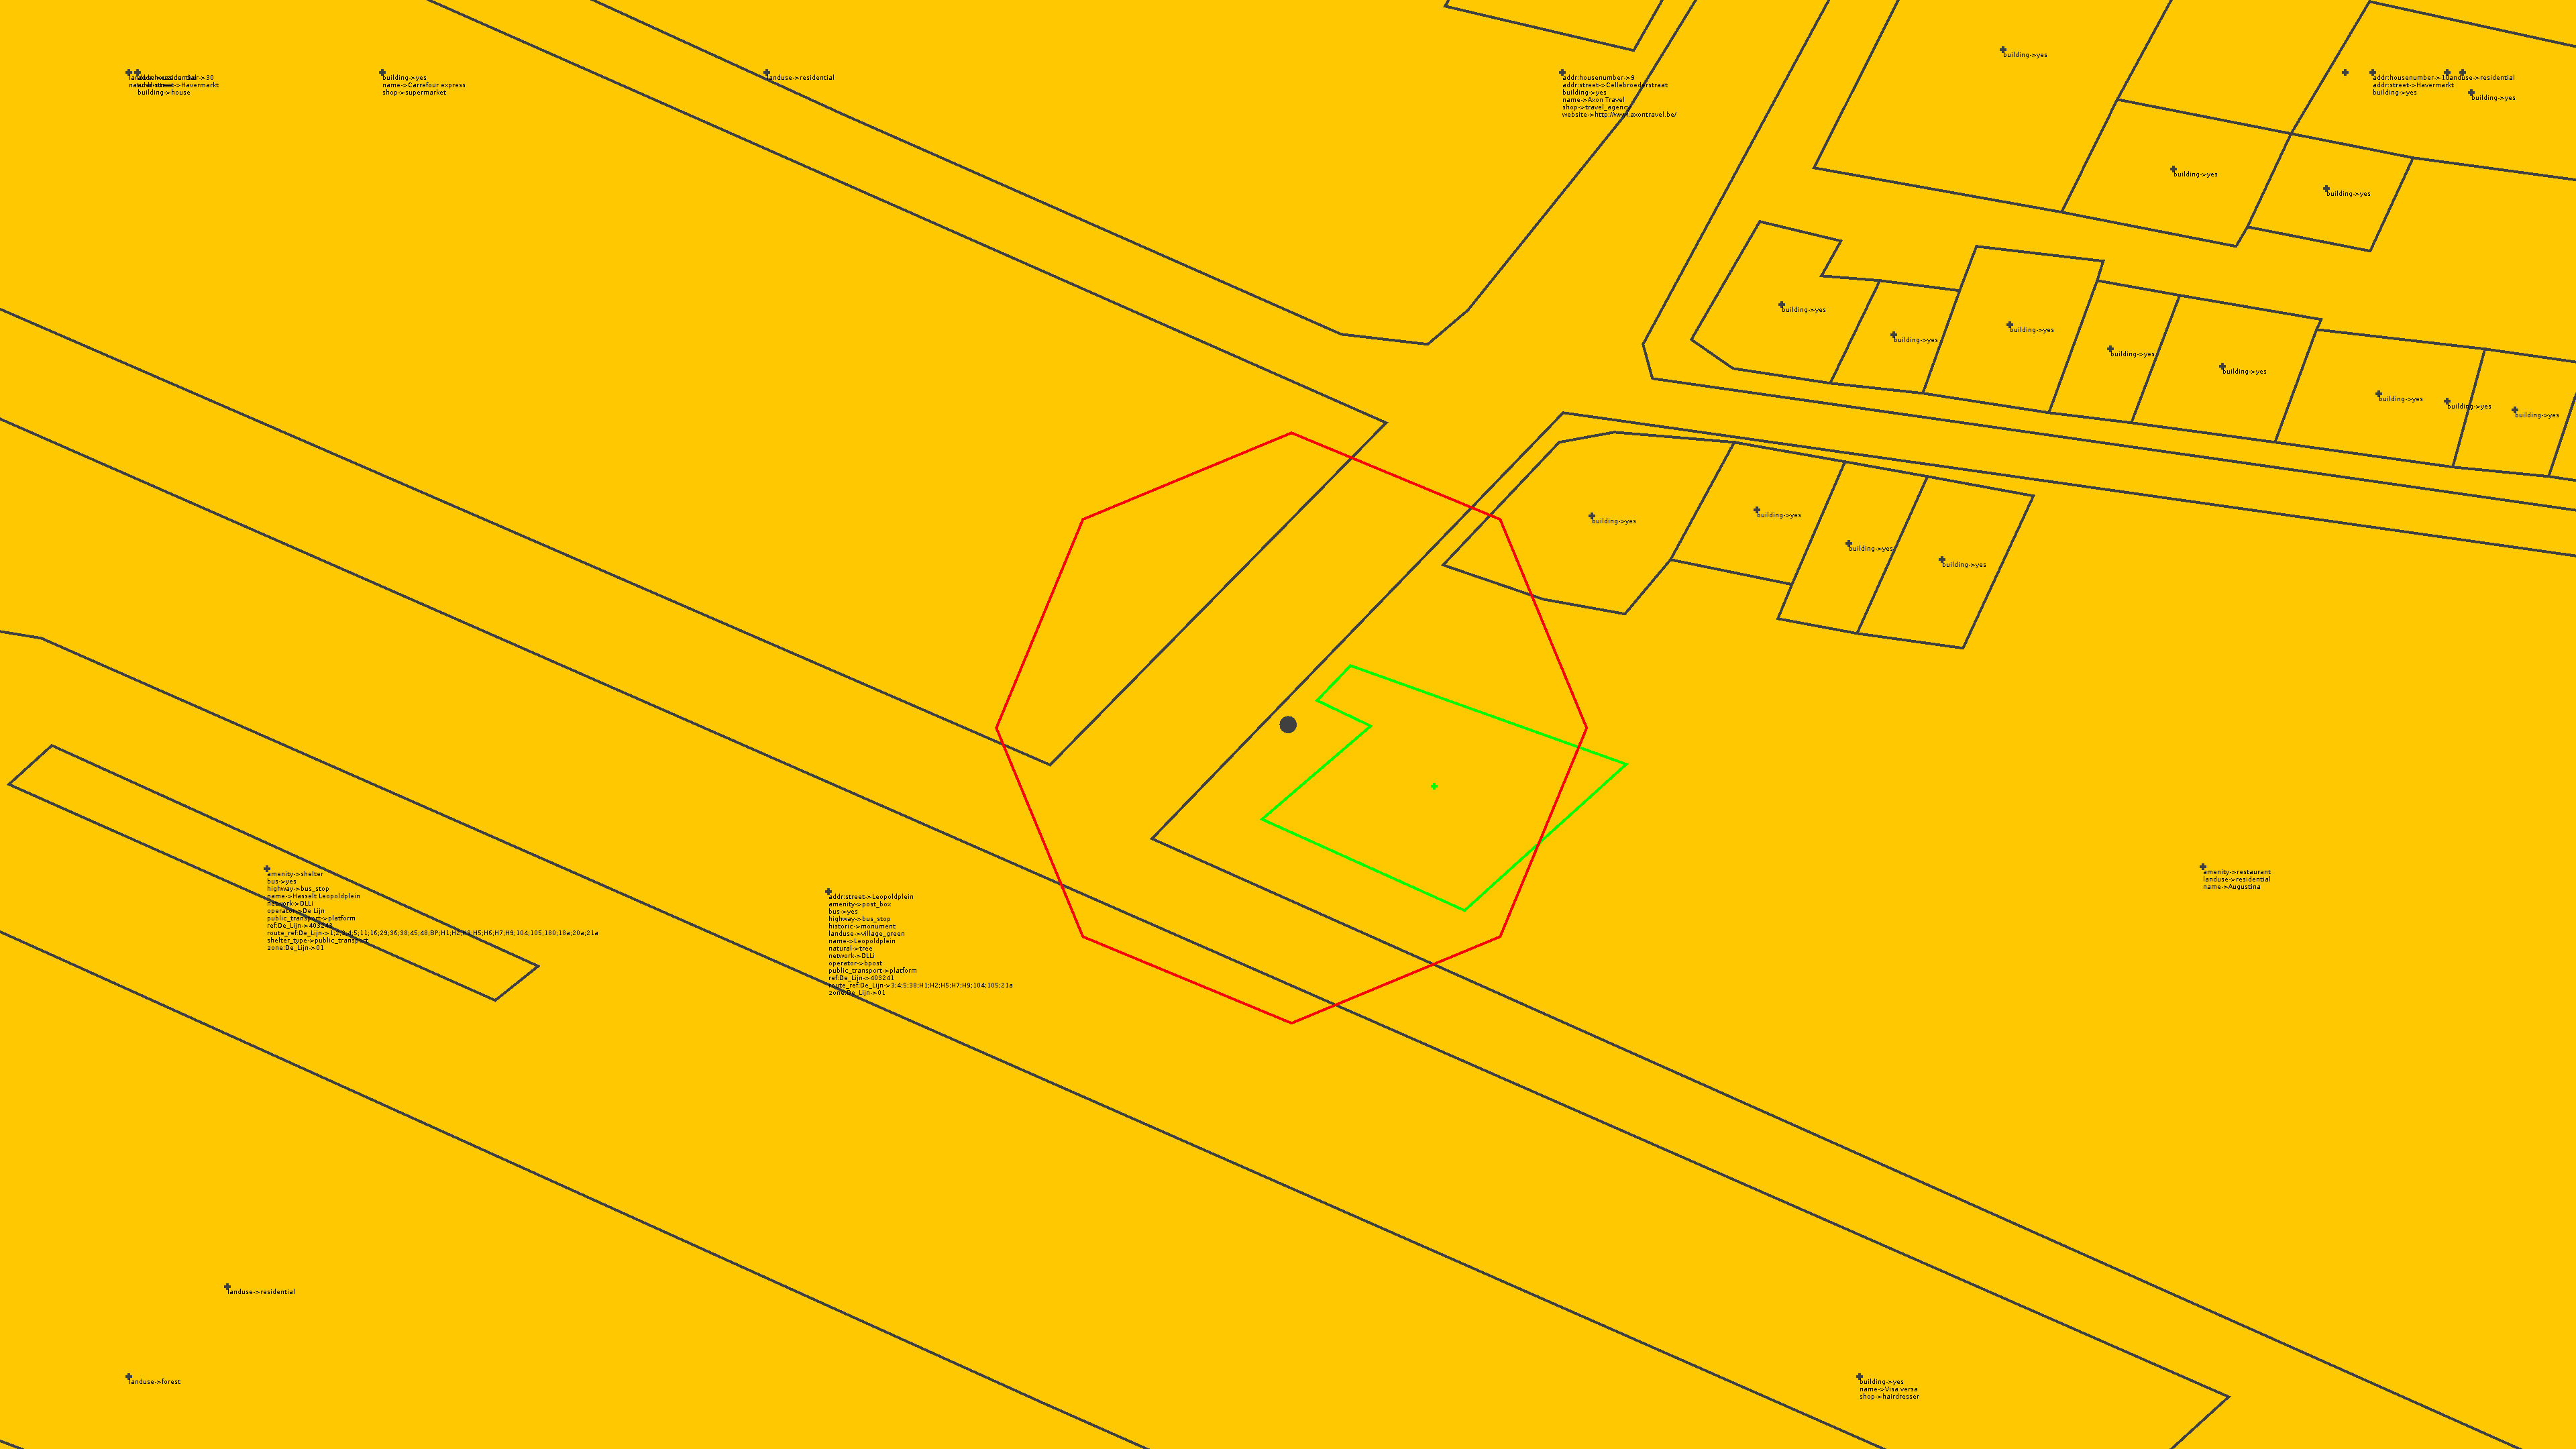
\includegraphics[width=\textwidth]{unvoll_full}}
\end{frame}


\begin{frame}
  \frametitle{Unvollständige Datensätze \hfill Nr. 38}
  \Wider{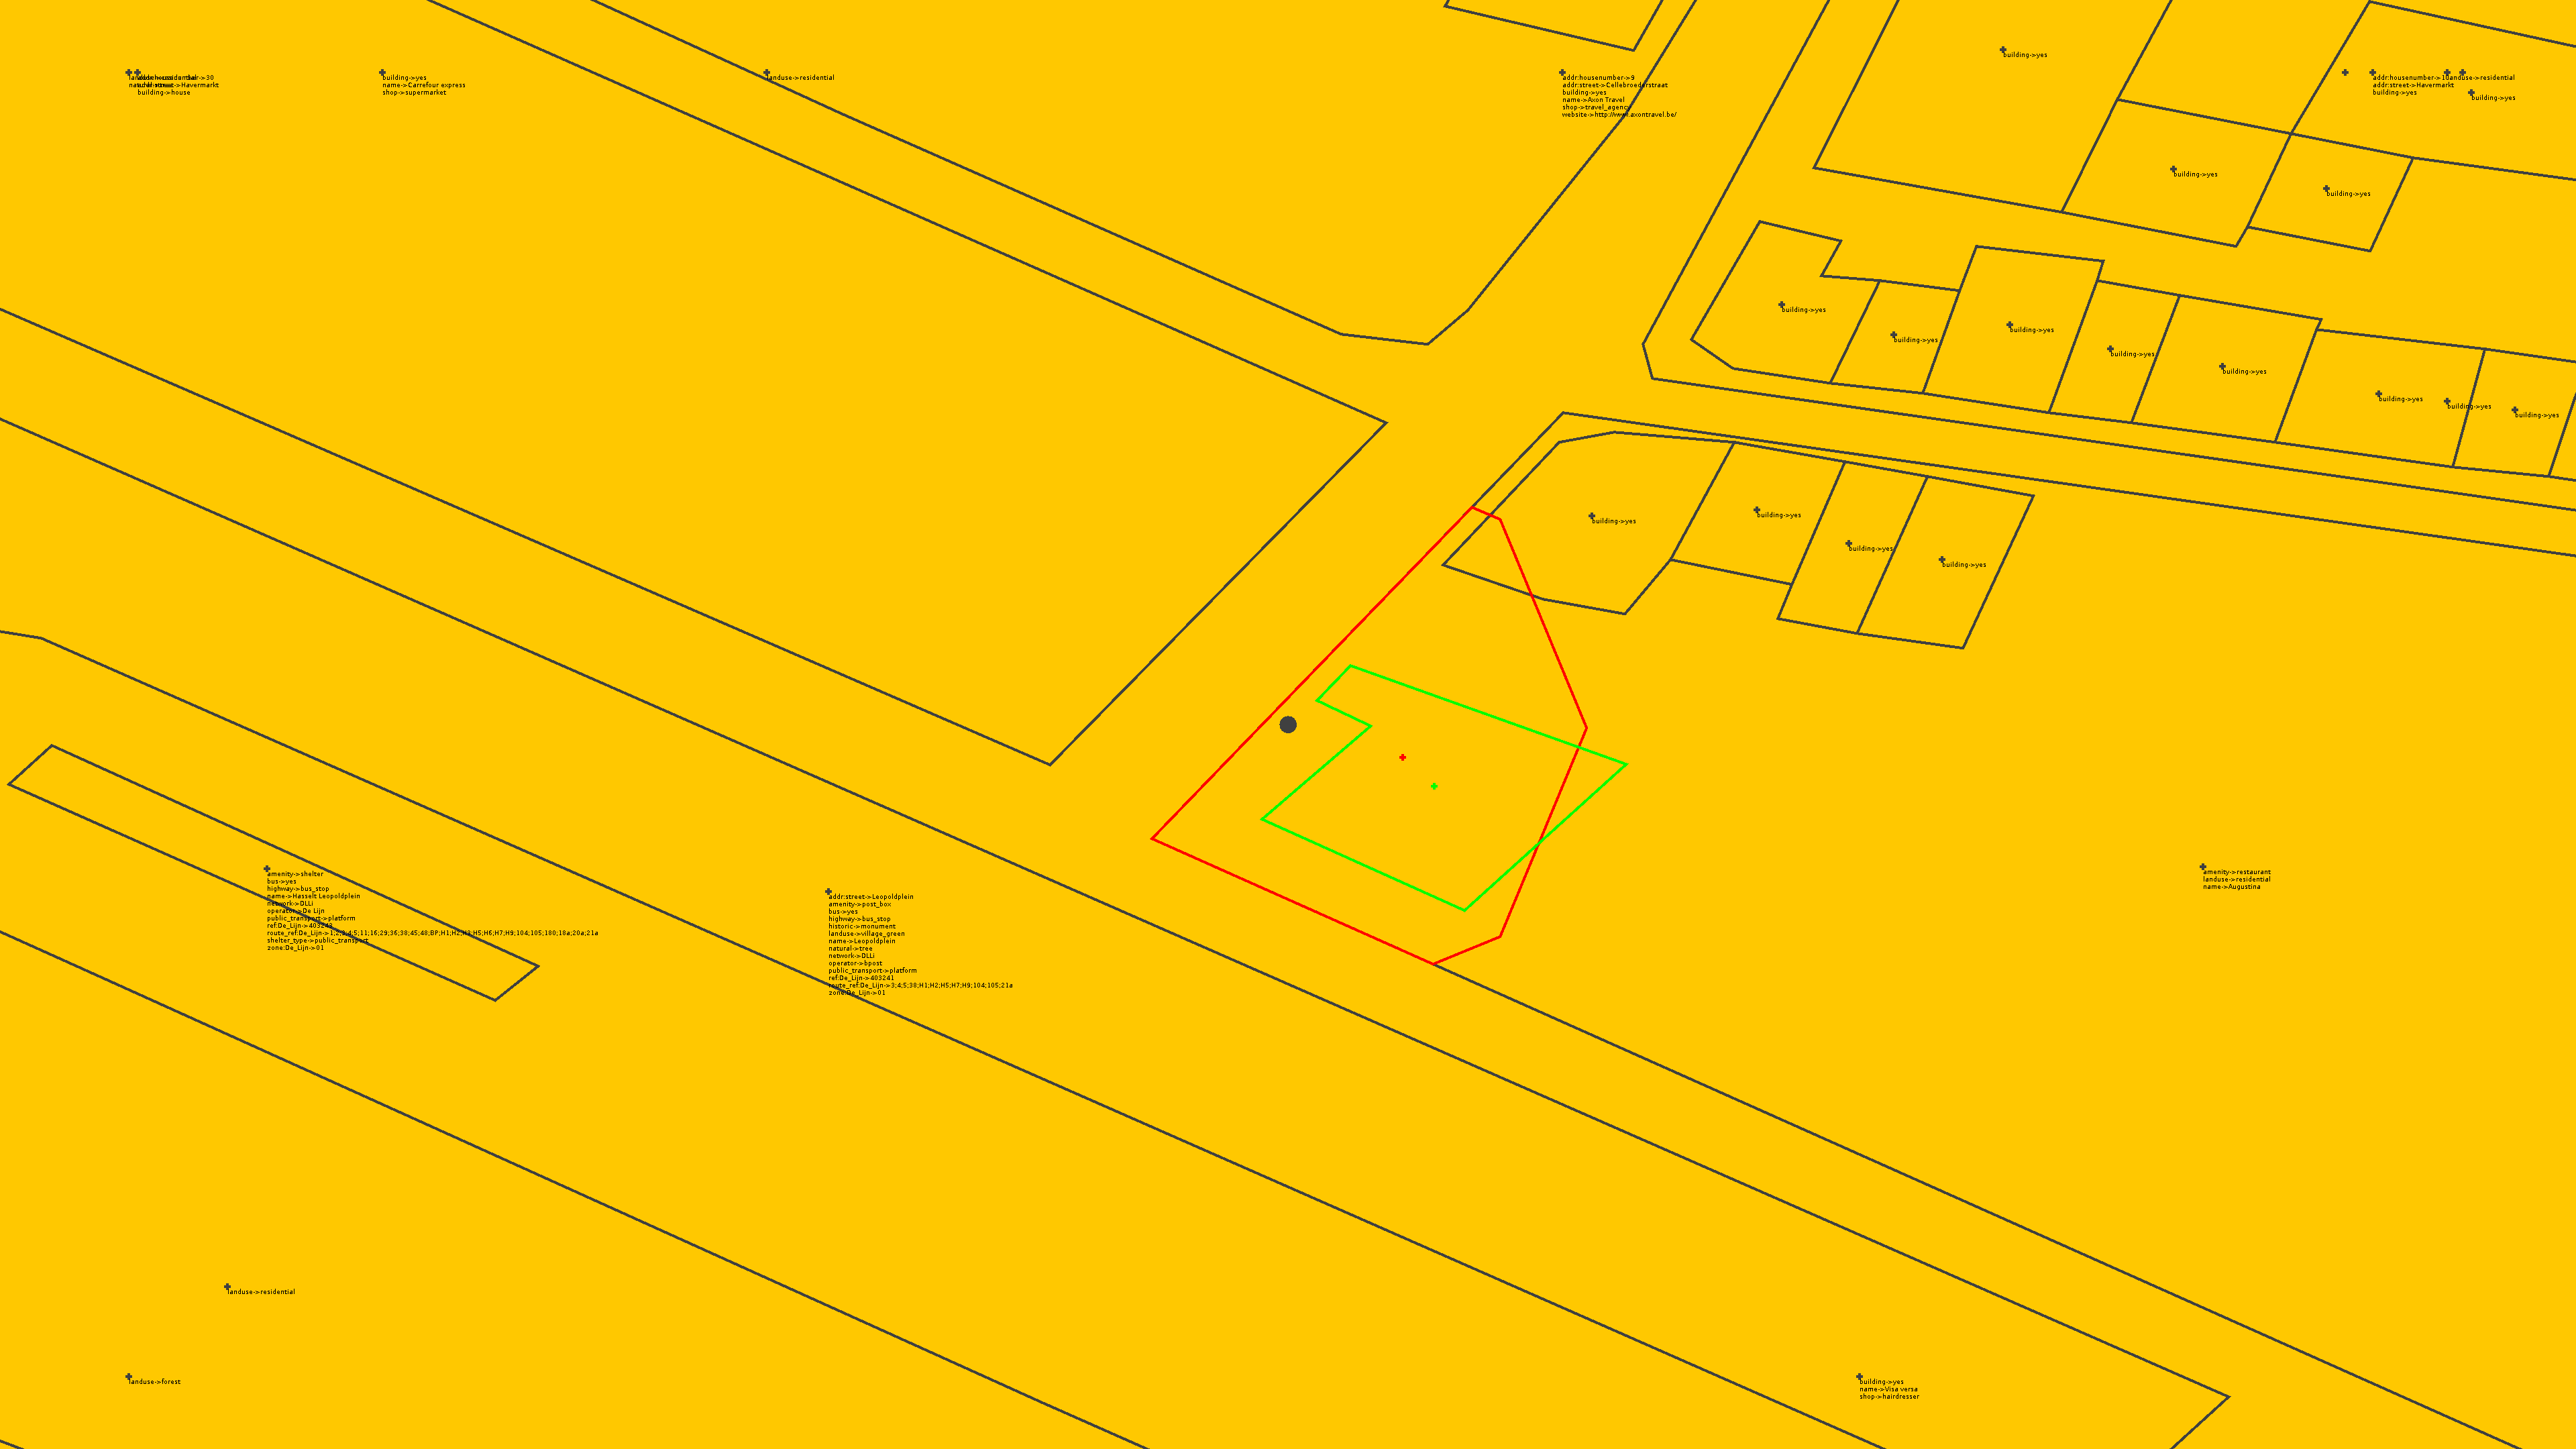
\includegraphics[width=\textwidth]{unvoll_result}}
\end{frame}

\begin{frame}
  \frametitle{Nicht implementiert \hfill Nr. 38}
  \Wider{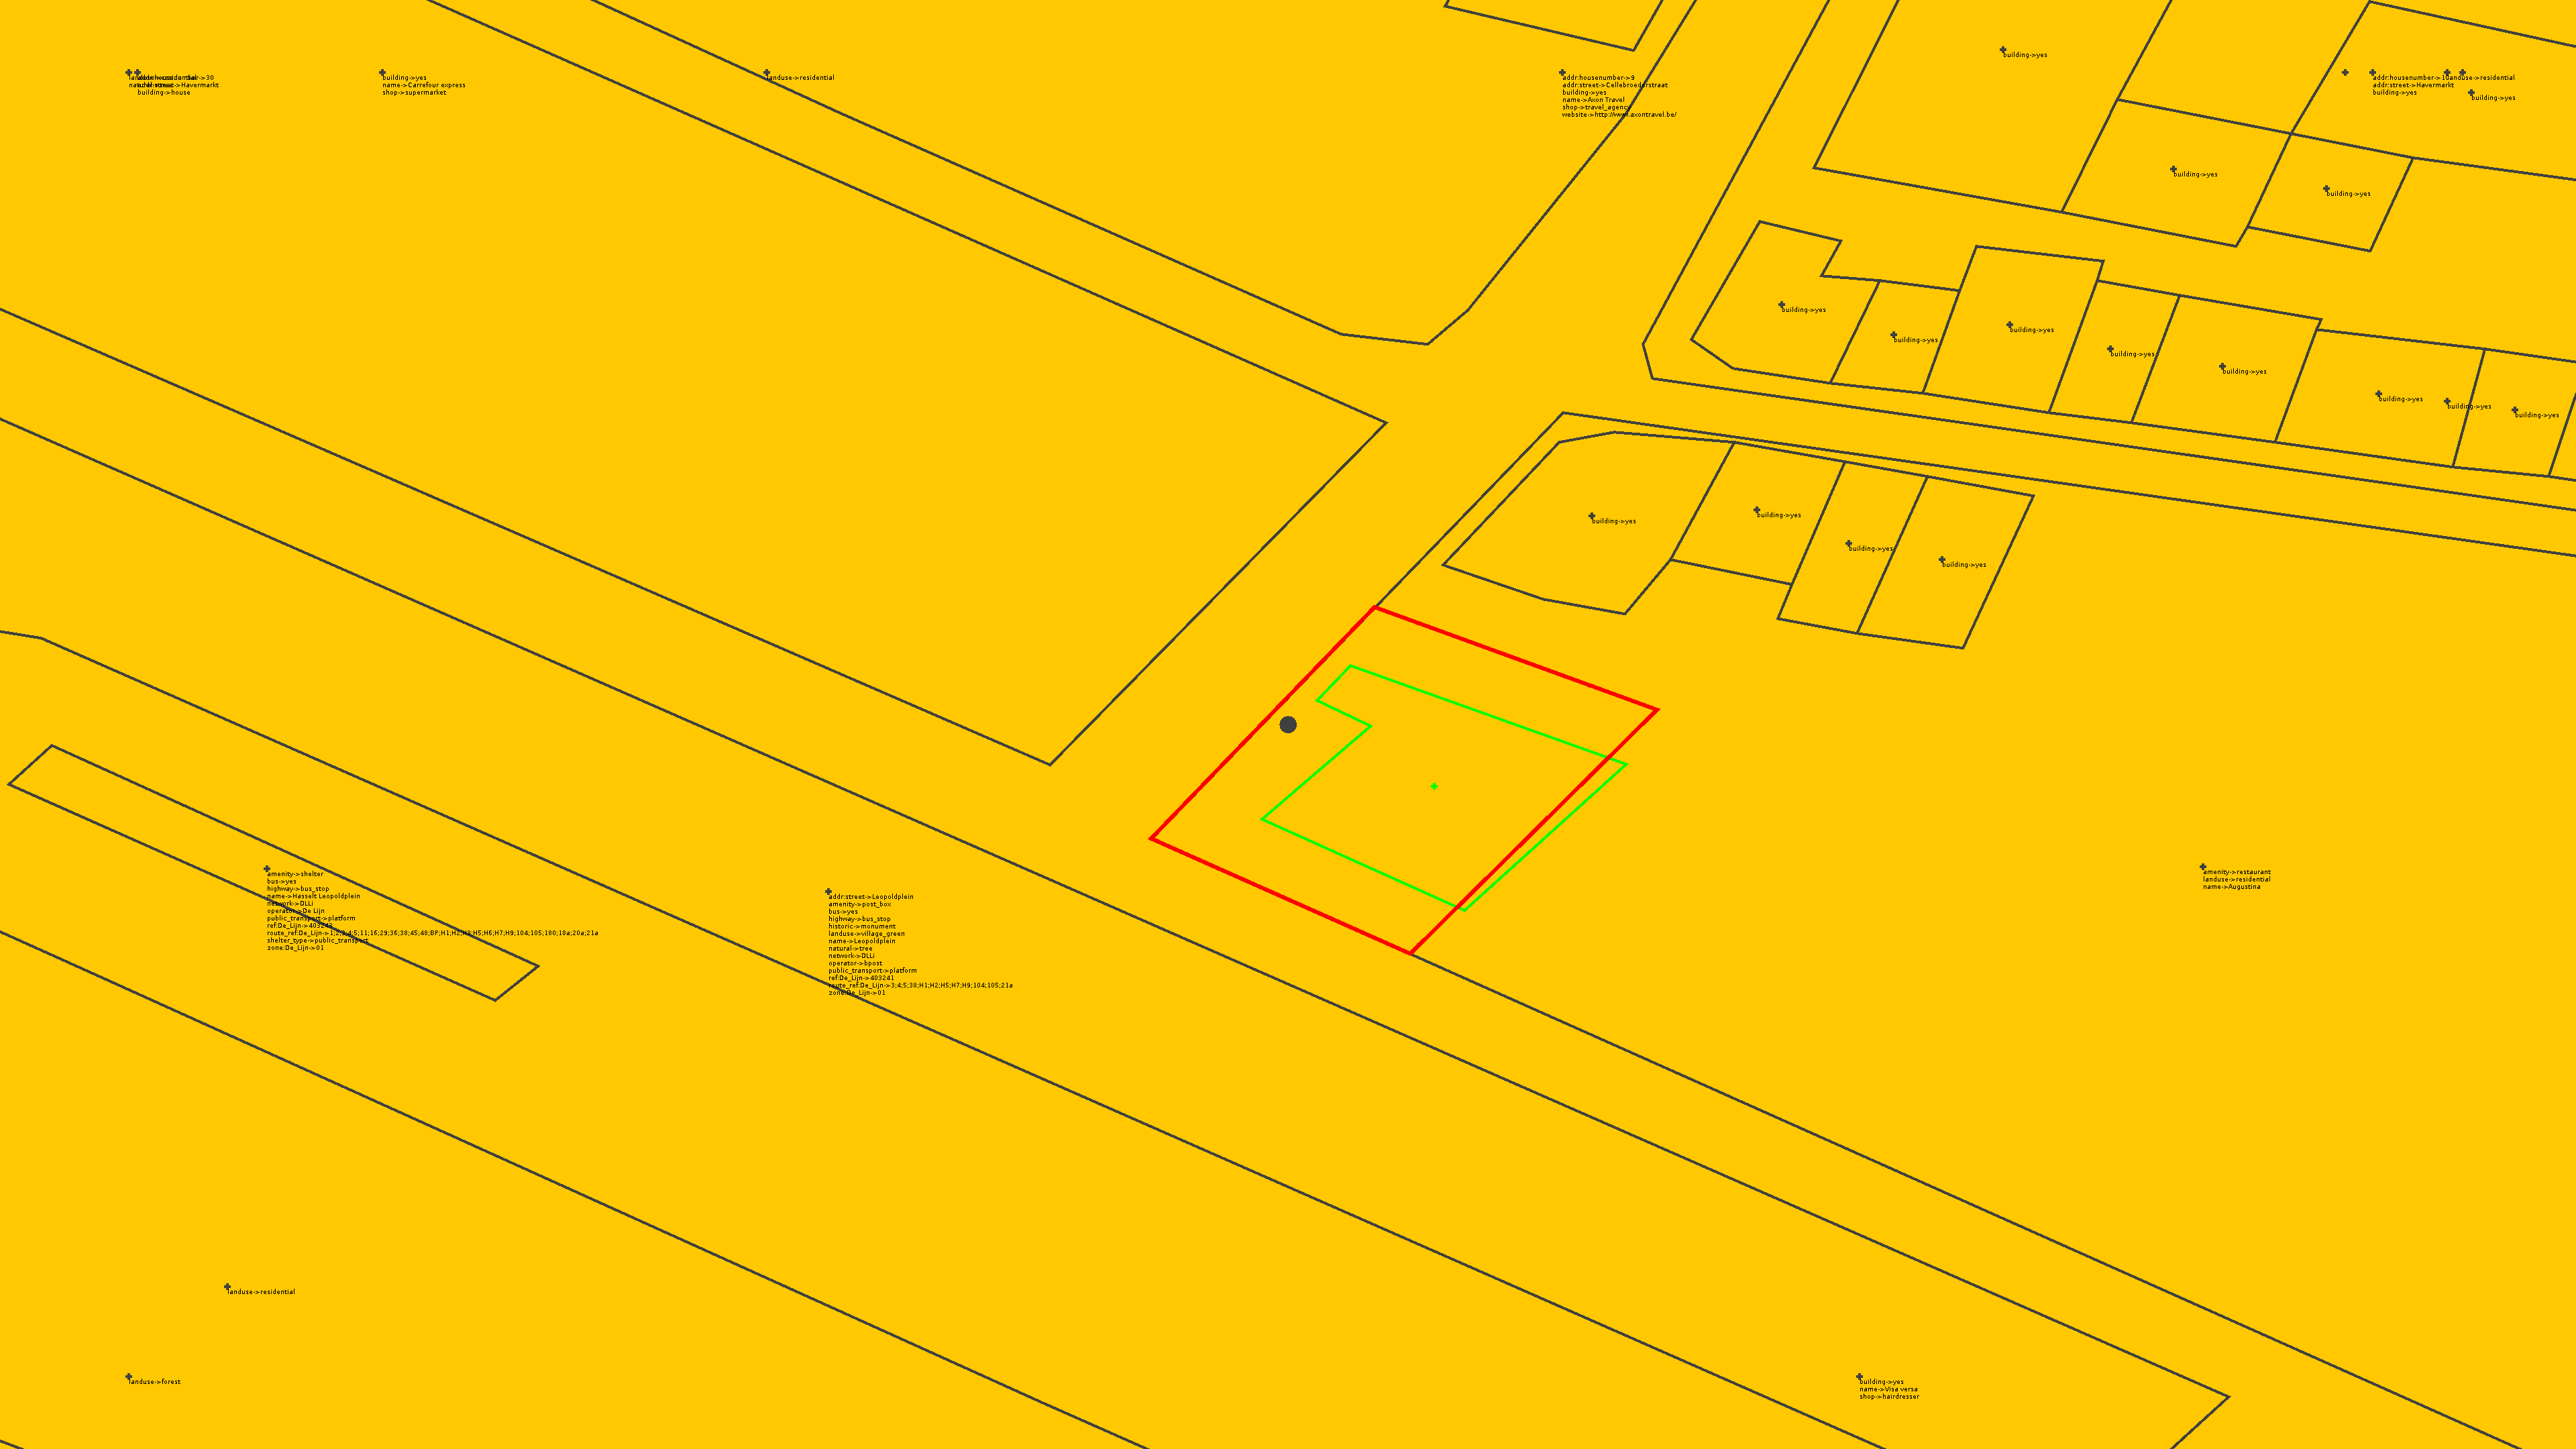
\includegraphics[width=\textwidth]{unvoll_parallel}}
\end{frame}


\begin{frame}
  \frametitle{Vollständiger Ansatz}
  \begin{center}
  \huge{Coverage = 74,6 \%}
  \end{center}
  \begin{center}
  Vorheriger Coverage =  69,8 \%
  \end{center}
\end{frame}

\begin{frame}
  \frametitle{Sonstige Verbesserungen}
  \begin{itemize}
    \item<1-> Partielle Gebäude zu einem zusammen gefügt
    \item<2-> OSM-Daten zwischengespeichert
    \item<3-> GPS-Daten aus Bildern auslesen
    \item<4-> GPS-Direction betrachtet (unnütz)
    \item<5-> Polygone erben Tags ihrer enthaltenen Punkte
    \item<6-> Multithreading
%%%%%%%%%%%%%%%%%%%%%%%%%%%%%%%%%%%%%%%%%%%%%%%%%%%%%%%%%%%%%%%%%%%%%%%%%%%%%%%%
% Weitere Verbesserungen die wir gemacht haben, aber nicht groß erklären wollen.
%%%%%%%%%%%%%%%%%%%%%%%%%%%%%%%%%%%%%%%%%%%%%%%%%%%%%%%%%%%%%%%%%%%%%%%%%%%%%%%%
%    \item ...
  \end{itemize}
\end{frame}

\begin{frame}[fragile]
 \frametitle{Aufbau des Regelsatzes}
 \[
  \begin{array}{c}
  \text{Rule} \\[6pt]
  \overbrace{\hspace{284pt}}\\[4pt]
    \{ \text{restrictions} \}
    \hspace{50pt}
    \{ \text{tag} \to (\text{weight}~[,\text{threshold},\text{radius}]) \} \\[6pt]
    \begin{array}{l r}
      \overbrace{ \hspace{80pt} } \hspace{10pt} & \overbrace{ \hspace{200pt} }\\
      \text{dog\_waste=``no''} & \text{landuse-recreation\_ground} \mapsto (0.7) \\
      \text{littering=``no''} & \text{landuse-residential} \mapsto (0.9,10^{-8},2.3\cdot 10^{-4}) \\
      \text{noise=``no''} &
    \end{array}
  \end{array}
 \]
\end{frame}

\begin{frame}[fragile]
  \frametitle{rules.xml Format}
  \lstset{language=XML,basicstyle=\scriptsize}
  \lstinputlisting{Rules.xml}
\end{frame}
